% \documentclass{article}
\documentclass[runningheads]{llncs}
\usepackage[spanish,english,portuguese]{babel}

% Set page size and margins
% Replace `letterpaper' with `a4paper' for UK/EU standard size
\usepackage[a4paper,top=2cm,bottom=2cm,left=3cm,right=3cm,marginparwidth=1.75cm]{geometry}
\usepackage{amsmath}
\usepackage{graphicx}
\usepackage[colorlinks=true, allcolors=blue]{hyperref}
\usepackage[utf8]{inputenc}
\usepackage{csquotes}
\usepackage{natbib}
\usepackage{url}
\usepackage{hyperref}
% \usepackage{footmisc}

\usepackage{color}

\def \bchregi {\begin{color}{red}} 
\def \echregi {\end{color}}

\def \bchgon {\begin{color}{blue}} 
\def \echgon {\end{color}}

\def \bchedel {\begin{color}{cyan}} 
\def \echedel {\end{color}}

\def \bwarn {\begin{color}{yellow}} 
\def \ewarn {\end{color}}

\providecommand{\keywords}[1]
{
  \small	
  \textbf{\textit{Keywords---}} #1
}

%\title{Identificando dimensiones de calidad en repositorios de datos abiertos de investigación educativa}
\title{Open Educational Research Data: Are Repositories Delivering?}
% \author{Gonzalo Torterolo-Silva - ORCID https://orcid.org/0009-0003-5004-0342}
% \author{Regina Motz - ORCID https://orcid.org/0000-0002-1426-562X}
% \author{Edelweis Rohrer - ORCID https://orcid.org/0000-0002-8257-5291}
% \author{
%   Torterolo-Silva, Gonzalo\\
%   \texttt{https://orcid.org/0009-0003-5004-0342}
%   \and
%   Motz, Regina\\
%   \texttt{https://orcid.org/0000-0002-1426-562X}
%   \and
%   Rohrer, Edelweis\\
%   \texttt{https://orcid.org/0000-0002-8257-5291}
% }
% \institute{UdelaR}

\begin{document}
\selectlanguage{spanish}
\maketitle

\selectlanguage{spanish}
\begin{abstract}
Este artículo analiza los criterios que influyen en la selección de repositorios de datos de investigación por parte de investigadores educativos. Se destaca la creciente importancia del acceso público a los datos en el contexto de la ciencia abierta y se examinan los principios FAIR (Encontrables, Accesibles, Interoperables, Reutilizables) como guía para la gestión de datos. El estudio se basa en una metodología mixta, que incluye una revisión bibliográfica, una consulta a expertos y un análisis de catálogos de repositorios.
La revisión bibliográfica identificó factores clave como la reputación del repositorio, la facilidad de uso, la disponibilidad de metadatos y el cumplimiento de los principios FAIR. La consulta a expertos enfatizó la importancia de los identificadores persistentes, la sostenibilidad y la interoperabilidad de los repositorios. El análisis de catálogos reveló que FAIRSharing se destaca por su curaduría y calidad de datos, mientras que re3data es una fuente primaria de información.
El artículo concluye que los investigadores educativos necesitan herramientas y criterios claros para seleccionar repositorios adecuados. Se subraya la necesidad de repositorios que faciliten la interoperabilidad y que cuenten con apoyo institucional y asistencia técnica. El estudio proporciona información valiosa para promover la adopción de prácticas de datos abiertos en el campo de la investigación educativa.
      
% Finalmente, se destaca el rol del investigador como agente activo que colabora en la  democratización del conocimiento científico, promoviendo una cultura de datos abiertos en el ámbito educativo.\\
\end{abstract}
% Regi: 5 keywords de ERIC en espa`nol
% Gonzalo: No hay version en español de las keywords (ver por ej https://vocabularyserver.com/eric/index.php?tema=255&/archives), por lo que traduje a mi criterio
\keywords{herramientas-de-investigación, archivos, catálogos-en-linea, metadatos, uso-de-datos}


\selectlanguage{english}
\begin{abstract}
This article discusses the criteria that influence the selection of research data repositories by educational researchers. It highlights the growing importance of public access to data in the context of open science and examines the FAIR (Findable, Accessible, Interoperable, Reusable) principles as a guide for data management. The study is based on a mixed methodology, including a literature review, expert consultation and analysis of repository catalogs.
The literature review identified key factors such as repository reputation, ease of use, metadata availability, and compliance with FAIR principles. Expert consultation emphasized the importance of persistent identifiers, sustainability and interoperability of repositories. Catalog analysis revealed that FAIRSharing stands out for its curation and data quality, while re3data is a primary source of information.
The article concludes that educational researchers need clear tools and criteria for selecting appropriate repositories. It stresses the need for repositories that facilitate interoperability and that have institutional support and technical assistance. The study provides valuable information to promote the adoption of open data practices in the field of educational research.
\end{abstract}
% 5 keywords de ERIC
% https://vocabularyserver.com/eric/index.php?tema=6128&/research-tools
% https://vocabularyserver.com/eric/index.php?tema=255&/archives
% https://vocabularyserver.com/eric/index.php?tema=3223&/online-catalogs
% https://vocabularyserver.com/eric/index.php?tema=4001&/metadata
% https://vocabularyserver.com/eric/index.php?tema=5348&/data-use
\keywords{research-tools, archives, online-catalogs, metadata, data-use}


\selectlanguage{portuguese}
\begin{abstract}
Este artigo discute os critérios que influenciam a seleção de repositórios de dados de pesquisa por pesquisadores educacionais. Ele destaca a importância crescente do acesso público aos dados no contexto da ciência aberta e examina os princípios FAIR (Findable, Accessible, Interoperable, Reusable) como um guia para o gerenciamento de dados. O estudo baseia-se em uma metodologia mista, incluindo uma revisão da literatura, uma consulta a especialistas e uma análise de catálogos de repositórios.
A revisão da literatura identificou fatores importantes, como a reputação do repositório, a facilidade de uso, a disponibilidade de metadados e a conformidade com os princípios FAIR. A consulta a especialistas enfatizou a importância dos identificadores persistentes, da sostenibilidade e da interoperabilidade dos repositórios. A análise dos catálogos revelou que o FAIRSharing se destaca por sua curadoria e qualidade de dados, enquanto o re3data é uma fonte primária de informações.
O artigo conclui que os pesquisadores educacionais precisam de ferramentas e critérios claros para selecionar os repositórios adequados. Ele destaca a necessidade de repositórios que facilitem a interoperabilidade e que tenham apoio institucional e assistência técnica. O estudo fornece informações valiosas para promover a adoção de práticas de dados abertos no campo da pesquisa educacional.
\end{abstract}
\keywords{ferramentas-de-pesquisa, arquivos, catálogos-online, metadados, uso-de-dados}

\selectlanguage{spanish}
\section{Introducción}
\label{intro}
En la era digital actual, el movimiento de ciencia abierta ha reconfigurado profundamente los paradigmas de producción y circulación del conocimiento científico. Dentro de este marco transformador, el acceso público a los datos de investigación emerge como un componente estratégico fundamental, particularmente en el campo educativo. \  La aplicación de estos paradigmas no solo robustece los pilares de transparencia y reproducibilidad que sustentan el método científico \cite{oecd2020}, sino que además facilita el análisis secundario y contribuye al impacto social del conocimiento \citep{ec2016, wilkinson2016}. Los beneficios potenciales son particularmente significativos en el ámbito educativo, donde la posibilidad de contrastar resultados entre diferentes contextos socioculturales y sistemas pedagógicos podría generar insumos para la evolución de las políticas públicas en educación. 

La \citet[p.~10]{unesco2021} conceptualiza los datos abiertos de investigación como aquellos que deben estar ``disponibles de manera oportuna, en un formato fácil de utilizar, legible y modificable por personas y máquinas'', articulándose bajo los principios FAIR (Fáciles de encontrar, Accesibles, Interoperables y Reutilizables) \citep{wilkinson2016}.  La disponibilidad de repositorios alineados con estos principios facilita la tarea de los investigadores, tanto para depositar como para reusar datos. Sin embargo, no es trivial decidir en qué repositorio depositar, organizar y gestionar los datos de investigación. En este sentido, los principios TRUST \citep{Lin2020TRUST} representan un marco de referencia muy valioso para evaluar la calidad de los repositorios científicos,  promoviendo la Transparencia (políticas de uso claras), Responsabilidad (en lo que refiere a la gestión de las colecciones de datos), el foco en el Usuario (disponibilidad de  herramientas para explorar, ubicar y reusar datos), Sostenibilidad (disponibilidad de los servicios de acceso a los datos  a largo plazo) y Tecnología (uso e implementación de estándares y herramientas adecuadas para la gestión y curación de los datos).
La exhaustiva caracterización de \citep{behnke_2020_5361952} detalla cómo estos principios  incluyen tanto requerimientos organizacionales (como políticas claras de gestión de datos y soporte para formatos estándar) como técnicos (desde metadatos granularizados hasta sistemas de identificadores persistentes).  \\


La organización y agrupación de colecciones de datos de investigación en repositorios responde a diferentes criterios de acuerdo a los cuales es posible categorizar los repositorios como disciplinares, cuando contienen datos 
de un área específica de conocimiento, generalistas, en caso contrario, y también institucionales, en caso de albergar datos de una institución en particular. %o no,  y entre repositorios institucionales o huérfanos (contienen datos que no pertenecen a una institución en particular). 
A su vez, en algunas disciplinas, por ejemplo economía o epidemiología, la mayor parte de los datos gestionados son cuantitativos, mientras que en otras, como las ciencias sociales y la educación, los datos son en su mayor parte cualitativos. Cada una de estas categorías de repositorios puede requerir la priorización de algunos principios sobre otros, o el uso de diferentes estándares o tecnologías para su implementación. En general, los datos de investigación de una misma disciplina tienen características en común, por lo que los requerimientos tecnológicos son similares. %Por ejemplo, en algunas disciplinas los datos deben estar actualizados en todo momento, por lo que van a usar los mismos a estándares de metadatos. 
%ACA DECIR que en general los datos de una misma disciplina son de naturaleza similar (es verdad?), por ejemplo requieren del mismo tipo de metadatos (por ejemplo datos que deben estar siempre actualizados....o lo que más importa es la reputación de la fuente), entonces la plataforma tecnológica va a tener los mismos requerimientos....
En particular, la investigación educativa enfrenta obstáculos específicos, especialmente cuando se trabaja con datos cualitativos que, como destaca \citep{antonio}, demandan niveles excepcionales de contextualización y mecanismos especializados de protección ética, implementados con tecnologías específicas, que muchos repositorios generalistas no están preparados para ofrecer.   
Otros estudios como el de \citep{strecker_disappearing_repos_23} informan sobre los riesgos de estos repositorios para cumplir con los estándares de calidad, indicando además que los repositorios disciplinares afines a humanidades y ciencias sociales son de los más afectados por este tipo de problemas. Otros autores, como \citep{google_dataset_aglomeration} y \citep{ Gerasimov2024} también advierten sobre tendencias de centralización de la mayoría de los datasets sobre el conjunto de repositorios generalistas. Paradójicamente, varias recomendaciones de estos repositorios generalistas alientan a los investigadores a utilizar repositorios disciplinares e institucionales \cite{barbosa_2024_11105430}.
En particular, los trabajos de \citep{Jia25} y \citep{avila2024} destacan por su análisis exhaustivo de las pautas para seleccionar repositorios de datos científicos confiables. 
También organismos internacionales como la \cite{unesco2021} y la \cite{oecd2020}, alineados con los principios FAIR y TRUST, han impulsado políticas que fomentan el uso de repositorios digitales especializados para el almacenamiento, preservación y diseminación ética de datos científicos. 

Como argumentan \citep{borgman2018}, estas infraestructuras digitales han dejado de ser meros almacenes de información para convertirse en nodos fundamentales de las redes contemporáneas de producción de conocimiento, facilitando no solo el acceso sino también la interoperabilidad y el enriquecimiento progresivo de los datasets mediante sucesivas reutilizaciones. En esta misma línea, la reciente conceptualización de \citep[p.~27]{avila2024} enfatiza su rol como sistemas dinámicos que permiten ``almacenar, organizar, recuperar y acceder a conjuntos de datos de diversa naturaleza temática y tipológica'', constituyéndose así en motores esenciales para la ciencia abierta. \\

La aplicación de los principios FAIR \cite{wilkinson2016} y TRUST \cite{Lin2020TRUST}  enfrentan retos particulares en disciplinas como la educación y las ciencias sociales, donde la heterogeneidad, sensibilidad y complejidad de los datos dificultan la estandarización y la creación de infraestructuras especializadas, alineadas con los requerimientos de estas disciplinas. Sin embargo, la escasez de repositorios disciplinares en estas áreas, sumada a desafíos éticos, legales y culturales, obliga a los investigadores a recurrir mayoritariamente a repositorios institucionales o generalistas, que no siempre satisfacen los requerimientos específicos para la gestión óptima de datos educativos y sociales.

Como advierte \citep{borgman2016} en su análisis sobre las ecologías del conocimiento, los datos solo alcanzan su pleno valor científico cuando se integran en ecosistemas robustos que articulen coherentemente dimensiones técnicas, prácticas comunitarias e institucionales. Precisamente, esta articulación presenta desafíos particulares en el ámbito educativo y de ciencias sociales, donde la disponibilidad de repositorios disciplinares especializados es escasa en comparación con otras áreas del conocimiento \cite{kraehmer2023,Lamb2024}. Esta disparidad resulta paradójica si consideramos la complejidad intrínseca de los datos educativos, que abarcan desde mediciones cuantitativas estandarizadas hasta registros etnográficos profundamente contextualizados, frecuentemente conteniendo información sensible ( por ej. sobre menores de edad en entornos escolares específicos \cite{gomes2022}).\\
 
Frente a estos desafíos, iniciativas como re3data \cite{pampel2013} han buscado crear catálogos integrados que faciliten la localización y evaluación de repositorios especializados. La selección informada de repositorios se vuelve entonces un desafío crucial. Los catálogos de repositorios 
emergen como herramientas clave para buscar, filtrar y evaluar opciones según criterios técnicos, éticos y disciplinares. 

Sin embargo, referente a repositorios de datos de investigaciones en educación, se observa una muy  escasa presencia disciplinar. Como muestra la Fig.~\ref{catalogos} la cantidad de repositorios de datos etiquetados como de educación obtenidos en  los catálogos re3data, FAIRsharing y DataCite Commons son un muy bajo número respecto al número total de repositorios indexados.
En este sentido, creemos que este trabajo aporta en prestar atención a las necesidades de los investigadores de la educación, para continuar mejorando el servicio que los repositorios pueden ofrecerles, para incentivar así su desarrollo.

%Algunos catálogos permiten entender la capacidad de los repositorios para expresar, mediante el uso de estándares, el contexto de cada investigación, %(paradatos), de manera est´andarizada haciendo que sus datos sean más fácilmente encontrables. Otros permiten descubrir la disponibilidad de servicios relacionados, como curaduría disciplinar, soporte, foros, entorno colaborativo o integración con redes sociales. 

\begin{figure}[h]
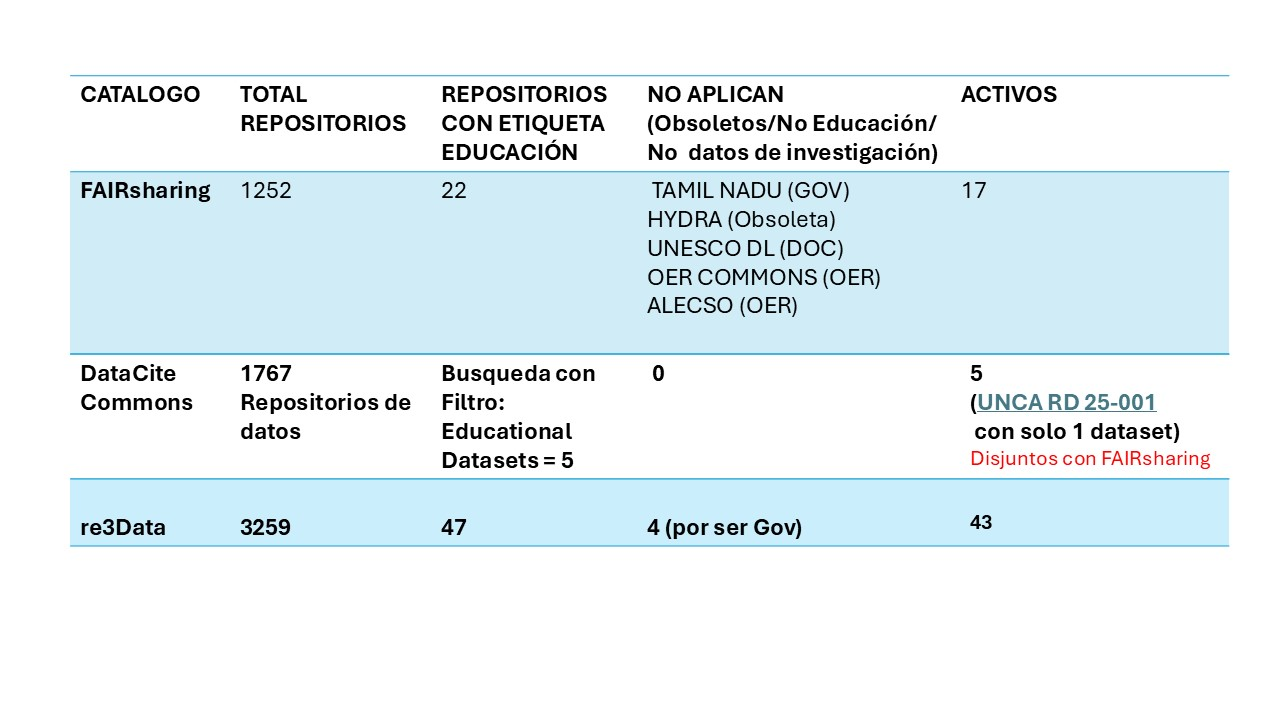
\includegraphics[width=0.9\textwidth]{catalogos.jpg}
\caption{Repositorios de datos de investigaciones educativas registrados en los catálogos al 26/6/2025} \label{catalogos}
\end{figure}

Este artículo analiza las necesidades para la publicación de datos en educación y ciencias sociales, y las características  de los repositorios más valorados por las investigadoras y los investigadores de estas disciplinas, considerando sus preocupaciones éticas, técnicas y legales. Además, este trabajo explora el papel de los catálogos de repositorios en la selección de repositorios como toma de decisiones informadas, con el objetivo de fortalecer la cultura de datos abiertos y contribuir al avance de la ciencia abierta en estas disciplinas.\\


%Esta aproximación normativa no solo robustece los pilares de transparencia y reproducibilidad que sustentan el método científico \cite{oecd2020}, sino que además facilita el análisis secundario y contribuye al impacto social del conocimiento \citep{ec2016, wilkinson2016}. Los beneficios potenciales son particularmente significativos en el ámbito educativo, donde la posibilidad de contrastar resultados entre diferentes contextos socioculturales y sistemas pedagógicos podría generar insights transformadores para las políticas públicas en educación.\\

%Ante este panorama promisorio, organismos internacionales como la \cite{unesco2021} y la \cite{oecd2020} han impulsado políticas que fomentan el uso de repositorios digitales especializados para el almacenamiento, preservación y diseminación ética de datos científicos. Como argumentan \cite{borgman2018}, estas infraestructuras digitales han dejado de ser meros almacenes de información para convertirse en nodos fundamentales de las redes contemporáneas de producción de conocimiento, facilitando no solo el acceso sino también la interoperabilidad y el enriquecimiento progresivo de los datasets mediante sucesivas reutilizaciones. En esta misma línea, la reciente conceptualización de \citet[p.~27]{avila2024} enfatiza su rol como sistemas dinámicos que permiten ``almacenar, organizar, recuperar y acceder a conjuntos de datos de diversa naturaleza temática y tipológica'', constituyéndose así en motores esenciales para la ciencia abierta.\\


%\bchgon
%Bien. Estadísticas "simples" se pueden obtener desde https://www.re3data.org/metrics/subjects . Sino puedo correr algunas consultas más elaboradas desde los datos crudos.
%\echgon


%Los principios FAIR \citep{wilkinson2016} y TRUST \citep{Lin2020TRUST} constituyen marcos de referencia valiosos para evaluar la calidad de los repositorios científicos. La exhaustiva caracterización de \cite{behnke_2020_5361952} detalla cómo estos incluyen tanto requerimientos organizacionales (como políticas claras de gestión de datos y soporte para formatos estándar) como técnicos (desde metadatos granularizados hasta sistemas de identificadores persistentes). Sin embargo, su implementación en investigación educativa enfrenta obstáculos específicos, especialmente cuando se trabaja con datos cualitativos que, como  destaca \cite{antonio}, demandan niveles excepcionales de contextualización y mecanismos especializados de protección ética que muchos repositorios generalistas no están preparados para ofrecer.\\

%No obstante, la aplicación de estos principios enfrenta retos particulares en disciplinas como la educación y las ciencias sociales, donde la heterogeneidad, sensibilidad y complejidad de los datos dificultan la estandarización y la creación de infraestructuras especializadas. La escasez de repositorios disciplinares en estas áreas, sumada a desafíos éticos, legales y culturales, obliga a los investigadores a recurrir mayoritariamente a repositorios institucionales o generalistas, que no siempre satisfacen los requerimientos específicos para la gestión óptima de datos educativos y sociales.\\

%Frente a estos desafíos, iniciativas como re3data \citep{pampel2013} han buscado crear catálogos integrados que faciliten la localización y evaluación de repositorios especializados.\\

%Frente a este panorama, la selección informada de repositorios se vuelve un desafío crucial. Los catálogos de repositorios, como re3data, emergen como herramientas clave para buscar, filtrar y evaluar opciones según criterios técnicos, éticos y disciplinares. Este artículo analiza las particularidades de la publicación de datos en educación y ciencias sociales, y explora el papel de los catálogos de repositorios en la toma de decisiones informadas, con el objetivo de fortalecer la cultura de datos abiertos y contribuir al avance de la ciencia abierta en estas disciplinas.\\

%\bchgon **********************************************************
%¿aca hay que explicar un poco más cual es la ventaja de utilizar catálogos para buscar donde publicar datos? podrían ser:\\
%\bchregi CÓMO DESDE LOS CATALOGOS SE PUEDE SABER LO QUE SIGUE?:\\ \echregi
%\bchgon Lo pongo linea a linea\\ \echgon
%- capacidad de los repositorios para expresar el contexto de cada investigación (paradatos), de manera estándarizada para que sean más fácilmente encontrables\\
%\hspace*{1cm} No hay una sola manera y hay diferentes niveles. Los metadatablocks de dataverse son un ejemplo de "interoperabilidad federada" (así se lo nombra en https://scispace.com/papers/fair-2-0-extending-the-fair-guiding-principles-to-address-2sa0tfp53f) que es un 1er nivel de estandarización, muy flexible pero que requiere crosswalks entre cada repositorio. Otra manera es usar DDI-codebook (eg DDI-codebook: https://ddialliance.org/hubfs/sites/default/files/ddi-lite.html) te permite describir, valga la redundancia, el codebook de un dataset, o sea, cosas como la metodología que se usó para recolectar los datos (2.3 method* del arbol de DDI-codebook)\\
%- conocer la interconexión de cada repositorio con diferentes comunidades para evitar publicar varias veces en diferentes lugares (agregadores)\\
%\hspace*{1cm}  esto es muy caso a caso. Algunos grandes agregadores como openaire o datacite publican los criterios (técnicos) bajo los cuales un repositorio puede ser indexado. DataCitationIndex publica una lista fija de repositorios cosechados. La información está disponible, pero no de manera estructurada\\
%- evaluar la adecuación del repositorio para el tipo de investigación realizada y sus datos generados (manejo de información privada, licencias soportadas, tiempo de preservación ofrecido, costos asociados, etc)\\
%\hspace*{1cm} mucha de este tipo de información está disponible como parte de las políticas de cada repositorio. Por supuesto, esa información pocas veces se encuentre estructurada, algunos casos puntuales los recopila ppalmente FAIRSharing (diría que es único que ofrece acceso estructurado a ésta información) pero son los menos\\
%- descubrir la disponibilidad de otros servicios relacionados dispuestos por los diferentes repositorios (curaduría disciplinar, soporte, foros, entorno colaborativo, integración con redes sociales, etc).\\
%\hspace*{1cm} estas son "cositas" que no se promocionan explícitamente y son dificiles de evaluar sino es mediante prueba y error o que forman parte de servicios extra que hay que contratar.
%\echgon
%%% **********************************************************************************

\section{Metodología}
\label{Metodo}
Para la realización de este estudio se siguió un diseño metodológico de enfoque secuencial exploratorio con las siguientes tres fases interrelacionadas: Revisión Bibliográfica, Entrevista a Experto y Análisis de Catálogos.

\paragraph{Objetivo:} Identificar cómo responden los repositorios a las preocupaciones  éticas, técnicas y legales que tienen las investigadoras y los investigadores en el momento de depositar datos de investigaciones educativas.

\paragraph{Fases Metodológicas}
\begin{itemize}
    \item [a)] Revisión Bibliográfica
    
Fuentes: Artículos en Scopus/WoS/ (keywords: "open data" + "education research" + "concerns"), informes de UNESCO y OECD. Criterios de exclusión: trabajos sobre repositories de recursos educativos abiertos y trabajos que solo consideran el acceso abierto a publicaciones de investigación.

Análisis: Codificación asistida con Elicit \footnote{Asistente de investigación con IA: https://elicit.com/} para categorizar preocupaciones recurrentes (ej. privacidad, propiedad intelectual, esfuerzo adicional).

Resultado esperado: Mapa conceptual de barreras documentadas en la literatura (2015–2025).

\item [b)]  Entrevista a Experto

Participante: Responsable del repositorio de datos abiertos de la Agencia Nacional de Investigación e Innovación (ANII) de Uruguay.

Protocolo: Entrevista semiestructurada (30–45 min) 

Análisis: Transcripción y codificación para rectificar o ratificar categorías revisadas en la literatura.

\item [c)] Análisis de Catálogos de Repositorios

    Muestra:  6 Catálogos de amplio uso internacional(OpenDOAR, ROAR, OpenAIR, Figshare,DataCite Commons
    
    Variables evaluadas:COMPLETAR

\end{itemize}

\paragraph{Triangulación y Validación:}
 La combinación de estos tres métodos, revisión bibliográfica, consulta a experto y análisis de catálogos, permitió triangular la información, aumentando la validez y confiabilidad de los resultados.



%El presente estudio se orienta a responder la pregunta de investigación: \textbf{¿qué características de un repositorio de datos de investigación son valoradas por los investigadores educativos al momento de publicar sus colecciones de datos?}. Para abordar esta interrogante, se diseñó una metodología mixta que integra enfoques cualitativos y cuantitativos, permitiendo una comprensión integral del fenómeno estudiado.\\

%\subsection{Revisión Bibliográfica}
%Se realizó una revisión de la literatura para identificar las necesidades y preferencias de los investigadores educativos en relación con la publicación de datos. Esta revisión se centró en estudios que abordan las barreras para el intercambio de datos, las estrategias propuestas para superarlas y los factores que influyen en la elección de repositorios por parte de los investigadores.\\
%La revisión bibliográfica incluyó la búsqueda y el análisis de artículos científicos, informes técnicos, libros y otras publicaciones relevantes en bases de datos académicas, bibliotecas digitales y repositorios institucionales. Se utilizaron términos de búsqueda como ``repositorios de datos de investigación'', ``gestión de datos'', ``ciencia abierta'', ``principios FAIR'', ``metadatos'', ``intercambio de datos'', ``barreras para compartir datos'' y ``criterios de selección de repositorios''.\\

%Estudios como el de \cite{barczak2022} señalan que, si bien la mayoría de los investigadores se muestran abiertos a compartir sus datos cuando se les solicita, el intercambio de datos no es una práctica generalizada. \cite{barczak2022} proponen que, para abordar esta problemática, se deben establecer mecanismos institucionales, como incentivos para el intercambio de datos y políticas de revistas que requieran la divulgación de datos para las publicaciones. También sugieren brindar apoyo administrativo a los investigadores en la preparación de los datos.\\

%Investigaciones centradas en el contexto educativo \bchgon decir que son en latinoamérica, o del LACLO para ser específicos \echgon, como la de \cite{casali2022open}, indican que existe un desconocimiento significativo sobre los repositorios de datos abiertos entre los investigadores del área. \cite{casali2022open} también identifican una actitud positiva de los investigadores hacia la publicación de sus datos, pero señalan la necesidad de políticas nacionales y programas institucionales que promuevan esta práctica. Además, destacan barreras como el tiempo y el esfuerzo requeridos para compartir los datos, la falta de financiamiento para la estandarización de los datos y las restricciones relacionadas con la seguridad y la confidencialidad de los datos.\\
%\bchgon ¿Agregar otros estudios que demuestren situaciones similares a nivel global o en otras regiones (eg: europa, brasil)? \echgon

%\subsection{Consulta a Expertos}

%Para complementar y enriquecer la revisión bibliográfica, se realizó una consulta semiestructurada a un experto en gestión de repositorios de datos, con amplia experiencia en la creación y administración de repositorios institucionales. Esta entrevista permitió obtener una perspectiva práctica y actualizada sobre los requerimientos, desafíos y expectativas de los investigadores al publicar datos, así como sobre las funcionalidades y limitaciones de las plataformas existentes.



%%%%%%%%%%%%%%%%%%%%%%%%%%%%%%%%%%
%\subsection{Análisis de repositorios disciplinares disponibles}

%\bchgon
%Emulando la situación que un investigador en el área de educación podría experimentar, se realizó una búsqueda (explicar términos utilizados) de repositorios disciplinares de datos de investigación para la disciplina en cuestión. El resultado arrojó muchas veces resultados no repositorios de REAs, repositorios de artículos.\\

%%%  VER  VER  VER %%%%%%%%%%%%%%%%%%%%%%%%%%%%%%%%%%%%%%%%%%%%%%%%%%%%%%%%%
%Dentro de los repositorios de datos de investigación, la mayoría de los resultados obtenidos consitió en repositorios generalistas.\\

%Frente a la escasez de repositorios declarados como "de educación" o al menos "ciencias sociales" la opción de utilizar repositorios enfocados en "datos cualitativos".\\

%Otros estudios como \citet{devriendt2021} y \citet{prosser2022} siguen objetivos similares enfocados en el área disciplinar de las ciencias sociales y resaltan la mayor presencia de estudios cualitativos en esta área.\\

%==================================================
%lo que sigue se movió a resultados de la revisión bibliografica

%Los investigadores cualitativos en el área de ciencias sociales mencionan temas relativos a la privacidad de sus datos y el compromiso ético que implica su publicación. En ciencias sociales, los datos suelen involucrar personas, y aunque se anonimicen, muchos investigadores temen que los participantes puedan ser reidentificados, especialmente en comunidades pequeñas o temas sensibles \citep{kraehmer2023}. A pesar de existir mecanismos para mitigarlo, como el consentimiento informado, la responsabilidad de los repositorios en cuanto a la custodia de los datos no siempre resulta fácil de comprender para los productores de datos \citep{prosser2022}.\\

%Estudios recientes como el de \cite{Lamb2024} ratifican algunos desafíos propios de las investigaciones cualitativas. Los investigadores cualitativos destacan que los datos (como entrevistas o diarios de campo) necesitan un conocimiento contextual profundo para ser interpretados adecuadamente, algo difícil de transmitir al abrir los datos.\\
%=================================================
%%%%%%%    ver VER  VER VER  
%No es raro que también los investigadores tengan recomendaciones sobre donde depositrar sus datos desde revistas o founders (nature (https://www.nature.com/sdata/policies/repositories), PLOS (https://journals.plos.org/plosone/s/recommended-repositories) y NIH (https://sharing.nih.gov/data-management-and-sharing-policy/sharing-scientific-data/selecting-a-data-repository)). Este sería otro insumo para las busquedas de repositorios que los investigadores suelen considerar.

%De las busqueda anterior, algunos de los repositorios encontrados fueron QDR, icpsr, openICPSR, ldbase, Harvard Dataverse (corroborar busqueda, pero seguro algunas de estas va a aparecer)\\
%\echgon

%%%%%%%%%%%%%%%%%%%%%%%%%%%%%%%%%%%%%%%%%%%%%%%%%%%%%%%%%%
%\subsection{Análisis de Catálogos de Repositorios}

%Se llevó a cabo un análisis comparativo de los principales catálogos de repositorios de datos, con el objetivo de evaluar las características técnicas, organizativas y funcionales que los catálogos permiten conocer sobre los repositorios. Algunas de estas características (certificaciones, sostenibilidad) se comprenden mucho mejor mediante estos catálogos de repositorios. Otras características, como resumen de los contenidos de cada repositorio, pueden conocerse en cada caso, pero son presentadas de manera centralizada por los catálogos para una comparativa efectiva.\\

%Los catálogos analizados fueron:
%\bchregi
%Revisar redacción de presentación de catálogos. Agregar información que cada uno brinda
%\echregi
%\bchgon
%Pero descubrir la información que brinda cada uno no sería parte de lo hallazgos? Me entrevera un poco tener ésta sección tanto en método como en resultado (casi que la sacaría). Aquí creo que solo haría falta mencionar los catálogos y casi que textual como se declaran a ellos mismos solo para presentarlos. La información de como se indexan entre ellos es irrelevante\\
%\echgon

%\subsection{Triangulación y Validación}
%La combinación de estos tres métodos, revisión bibliográfica, consulta a experto y análisis cuantitativo de catálogos, permitió triangular la información, aumentando la validez y confiabilidad de los resultados. Este enfoque metodológico integral facilitó la identificación de criterios técnicos y prácticos relevantes para la selección de repositorios, alineados con las necesidades reales de los investigadores educativos y las mejores prácticas internacionales en gestión de datos.\\
%En conjunto, esta metodología robusta garantiza que las conclusiones y recomendaciones derivadas del estudio estén fundamentadas en evidencia diversa, actualizada y pertinente, contribuyendo así a fortalecer la infraestructura y cultura de datos abiertos en la investigación educativa.\\

\section{Resultados}

Esta sección presenta los resultados obtenidos a partir de la revisión bibliográfica, la consulta a expertos y el análisis de catálogos de repositorios.

\subsection{Resultados de revisión bibliográfica}

Numerosos estudios se han centrado en identificar los factores que impactan en la voluntad de los investigadores en compartir sus datos en abierto y se ha hecho un esfuerzo por destacar algunos de ellos aquí, especialmente desde la perspectiva de los repositorios. 
La revisión bibliográfica realizada muestra que los estudios abarcan encuestas, revisiones sistemáticas de la literatura, meta-análisis, grupos focales y mesas redondas, de las más actuales \citep{tenopir2011,revision2020,barczak2022,casali2022open, researchers2022,borycz2023,logan2021,researchers2024,malasya,bio-uy}. Es interesante observar que los estudios son con investigadores de distintas disciplinas, distinto nivel de expertise y de diferentes contextos geográficos. Curiosamente, pocos de estos estudios se han realizado con investigadores de Ciencias de la Educación. Entre los más destacados que involucran opiniones de investigadores relacionados con la disciplina Educación encontramos el trabajo de \citet{casali2022open} que analiza una encuesta administrada a investigadores de la comunidad LACLO (Conferencia Latinoamericana de Tecnologías de Aprendizaje) y los trabajos de \cite{logan2021} y de \cite{guia} 
que presentan guías sobre publicación de datos abiertos expresamente dirigidas para investigadores en Educación.\\

Mientras que el trabajo de \cite{casali2022open} destaca barreras como el tiempo y el esfuerzo requeridos para compartir los datos, la falta de financiamiento para la estandarización de los datos y las restricciones relacionadas con la seguridad y la confidencialidad de los datos, observamos que en los trabajos de \cite{logan2021, guia} se presta especial atención a los procedimientos para mantener la seguridad y la confidencialidad de los datos, evidenciando que este constituye un problema en común.\\

La mayoría de los trabajos coinciden en reconocer como aspectos importantes en la problemática planteada por los investigadores el esfuerzo extra que significa curar los datos para su publicación en abierto.  Mientras en general se atribuye esta problemática al desarrollo de los repositorios poco centrados en el usuario, para otros autores como \citet{borycz2023} y \citet{casali2022open}, se debe a la falta de apoyo administrativo a los investigadores en la preparación de los datos.\\

Otros estudios, como el de \citet{grattarola2024gaps} y \citet{ mabile2025recommendations}, señalan que la desmotivación principal para compartir los datos en abierto  recae en la falta de incentivos institucionales y la falta de reconocimiento por la publicación de datos.
Respecto al caso específico de datos procedentes de investigaciones cualitativas, se destaca en todos los trabajos la problemática de contar con elementos que permitan especificar el contexto en el cual los datos fueron obtenidos y la preocupación por contar con curaduría específica para asegurar el resguardo del investigador ante el problema legal y ético de uso de datos sensibles.\\

Los investigadores cualitativos en el área de ciencias sociales mencionan temas relativos a la privacidad de sus datos y el compromiso ético que implica su publicación. En ciencias sociales, los datos suelen involucrar personas, y aunque se anonimicen, muchos investigadores temen que los participantes puedan ser reidentificados, especialmente en comunidades pequeñas o temas sensibles \citep{kraehmer2023}. A pesar de existir mecanismos para mitigarlo, como el consentimiento informado, la responsabilidad de los repositorios en cuanto a la custodia de los datos no siempre resulta fácil de comprender para los productores de datos \citep{prosser2022}.\\

Estudios recientes como el de \cite{Lamb2024} ratifican algunos desafíos propios de las investigaciones cualitativas. Los investigadores cualitativos destacan que los datos (como entrevistas o diarios de campo) necesitan un conocimiento contextual profundo para ser interpretados adecuadamente cuando otros investigadores deciden reusar el dataset. \\

%algo difícil de transmitir al abrir los datos.
%\bchedel o en los propios datos abiertos? \echedel
%\bchgon tampoco me queda claro ¿será al publicar los datos? O se refiere a las %descripciones (readme.txt) de los datos que se incluyen por fuera de los metadatos y dentro de las colecciones? \echgon



\subsection{Resultado consulta a experto}

Las conclusiones derivadas de la entrevista con el experto se basan en un estudio interno realizado por la Agencia Nacional de Investigación e Innovación (ANII). Este estudio, aunque no publicado, proporcionó información valiosa sobre las perspectivas de los investigadores en el contexto de Uruguay.
El estudio de la ANII reveló que los investigadores tienden a percibirse principalmente como consumidores de datos, más que como productores. Esta percepción influye en sus expectativas y necesidades en relación con los repositorios de datos.
El experto entrevistado, basándose en los resultados del estudio, destacó tres características clave que los investigadores consideran esenciales al momento de publicar sus datos:
\begin{itemize}
    \item \textbf{Asignación de identificadores persistentes}: La asignación de identificadores únicos y permanentes, preferentemente DOI, es vista como un requisito fundamental, especialmente debido a que muchas revistas científicas los exigen para la evaluación y citación de artículos.
    \item \textbf{Sostenibilidad y perdurabilidad}: La capacidad del repositorio para garantizar la conservación de los datos a largo plazo es considerada crucial para asegurar su disponibilidad y reutilización futura.
    \item \textbf{Interoperabilidad}: La capacidad del repositorio para facilitar la integración y el intercambio de datos entre diferentes plataformas y sistemas es valorada como esencial para maximizar el impacto y la reutilización de los datos.
\end{itemize}

La modalidad semiestructurada de la entrevista facilitó la exploración profunda de temas relevantes, sin restringir la espontaneidad del diálogo, lo que contribuyó a validar y ampliar los resultados del relevamiento bibliográfico con evidencia empírica y experiencia directa.

\subsection{Resultado del análisis de catálogos de repositorios}
Los estudios de \citep{witt_2024_11221855} y \citep{Jia25} establecen los principales criterios para evaluar repositorios de datos de investigación; no obstante, señalan que los investigadores enfrentan obstáculos para verificar el cumplimiento de dichos criterios, dada la escasa accesibilidad de esta información a priori. Esta limitación dificulta la selección de un repositorio adecuado para la publicación y la reutilización de datos. En este trabajo, analizamos el papel de los catálogos de repositorios en la difusión eficiente de dicha información, tomando como referencia los criterios definidos por estos autores y los desarrollados en el Data Repository Attributes Working Group\footnote{\url{https://www.rd-alliance.org/groups/data-repository-attributes-wg/}}.
Las características que buscamos identificar son; creación de identificadores persistentes, soporte para especificar el contexto, cumplimiento de estándares para interoperabilidad y adhesión a políticas de licenciamiento y sostenibilidad.

\subsection*{Creación de identificadores persistentes} 

El Identificador Digital de Objeto (DOI, por sus siglas en inglés) desempeña un papel fundamental en los repositorios de datos de investigación, ya que garantiza la localización, citación y preservación permanente de los conjuntos de datos. Proporciona un enlace único y estable, evitando la pérdida de datos debido a cambios en las URL o la desactualización de repositorios. Esto asegura que los conjuntos de datos permanezcan accesibles a largo plazo, cumpliendo con los principios FAIR. Al integrarse con sistemas de gestión bibliográfica (como Crossref o DataCite), el DOI permite vincular conjuntos de datos con artículos científicos, mejorando su visibilidad y facilitando el seguimiento de su impacto.

El DOI (Digital Object Identifier) es asignado por agencias registradoras autorizadas, siendo DataCite la más utilizada para datos de investigación o por repositorios/instituciones afiliadas a DataCite. En algunos casos puede ocurrir que un mismo dataset termine teniendo múltiples DOIs. Esto puede ocurrir si un investigador carga el mismo dataset en distintos repositorios y cada uno le asigna un DOI distinto, o en caso de actualizaciones o versions, ya que algunos repositorios generan un nuevo DOI para versiones corregidas o ampliadas del mismo dataset. Esto no es deseable ya que las citas al dataset se dispersan entre varios DOIs, subestimando su impacto real y además se dificulta identificar cuál es la versión más actualizada. Para evitar estos problemas se recomienda priorizar el uso de repositorios de referencia en cada disciplina (ej. ICPSR en ciencias sociales) para evitar duplicaciones. En caso de esto no ser posible, las soluciones recomendadas son usar repositorios que admitan versiones bajo un mismo DOI y vincular DOIs alternativos mediante metadatos (relaciones \emph{isVersionOf} o \emph{isIdenticalTo} en esquemas como Schema.org). 

\subsection*{Soporte para documentar el contexto}

El contexto de un dataset incluye detalles sobre su origen, metodología con la cual fue generado, uso potencial y limitaciones. Los repositorios recolectan la información de contexto a través de metadatos descriptivos, documentación técnica (como Protocolos de laboratorio, cuestionarios o scripts de procesamiento), documentos adicionales (como Readme, Guías e Informes) y publicaciones vinculadas (DOI de artículos relacionados que usaron/citaron el dataset.)

En los metadatos descriptivos al menos se debe informar:  
\begin{itemize}
\item Origen: Quién lo creó (Institución, proyecto de investigación, autoría) y Cobertura temporal/geográfica (Cuándo y dónde se generó el dataset) 
\item Propósito: Objetivo de la recolección 
\item Métodos de recolección: Instrumentos, protocolos o software utilizados 
\item Licencias y restricciones: Condiciones de uso (CC-BY, GDPR, acceso restringido).
\end{itemize}

Para facilitar la interoperabilidad es una buena práctica usar vocabularios controlados
y ontologías disciplinares (por ej.:  OECD Education Taxonomy).\\



\bchregi -----------------revision DE ESTA SECCIÓN hasta acá--------------------------- \echregi \\

\bchregi mover a otro lado o que sigue o borrarlo \\


Los catálogos de repositorios de datos, como re3data, OpenAIRE, DataCite Commons, entre otros, son herramientas fundamentales en el ecosistema de la ciencia abierta y la gestión de datos de investigación. Estos catálogos actúan como índices o motores de búsqueda que permiten localizar repositorios de datos de investigación. En lugar de buscar de forma dispersa, los investigadores pueden utilizar estos catálogos para encontrar fuentes organizadas, de confianza y con políticas claras de acceso y preservación. Por ejemplo, DataCite Commons y re3data ofrecen interfaces de búsqueda que permiten filtrar y acceder a un gran volumen de registros de datos de investigación, lo que simplifica el proceso de encontrar información específica sin necesidad de conocimientos técnicos avanzados.\\

Los catálogos proporcionan información sobre las características de cada repositorio (licencias, políticas de preservación, acceso abierto, certificaciones, etc.), ayudando a seleccionar los que cumplen con los requisitos buscados por los investigadores.\\

Muchos de estos catálogos promueven el uso de estándares comunes en la descripción de repositorios y datos, lo cual facilita el descubrimiento automatizado de los repositorios y sus datasets, su vinculación con publicaciones científicas y la construcción de infraestructuras digitales integradas. \\

Los catálogos como OpenAIRE y DataCite Commons fomentan el uso de estándares internacionales (como el protocolo OAI-PMH y metadatos FAIR), lo que asegura que los datos sean fácilmente localizables, accesibles y reutilizables por diferentes plataformas y sistemas, favoreciendo la colaboración y el intercambio de información entre comunidades científicas.\\

Un aporte importante de los catalogos es que certifican repositorios: Evalúan criterios como interoperabilidad, licencias claras y metadatos estructurados (ej: FAIRsharing asigna sellos de cumplimiento FAIR).\\


Se llevó a cabo un análisis comparativo de los principales catálogos de repositorios de datos, con el objetivo de evaluar las características técnicas, organizativas y funcionales que los catálogos permiten conocer sobre los repositorios. 

%Algunas de estas características (certificaciones, sostenibilidad) se comprenden mucho mejor mediante estos catálogos de repositorios. 
%Otras características, como resumen de los contenidos de cada repositorio, pueden conocerse en cada caso, pero son presentadas de manera centralizada por los catálogos para una comparativa efectiva.\\


Se analizaron los siguientes catálogos:
\begin{itemize}
    \item 
\emph{OpenDOAR}: Directorio global de repositorios de acceso abierto que ofrece acceso a recursos y productos académicos, incluyendo repositorios de datos.
\item
\emph{ROAR}: Registro de repositorios de acceso abierto, con información recopilada de diversas fuentes, incluyendo OpenDOAR.
\item \emph{OpenAIRE}: Servicio que interconecta varios catálogos y proporciona información sobre las relaciones entre repositorios, autores, instituciones y agencias de financiación. Se especializa en el marco conceptual de la EOSC \bchregi decir lo que es EOSC \echregi y los servicios ofrecidos en su ecosistema.
\item 
\emph{FAIRsharing}:  Portal web que describe estándares, bases de datos y políticas de datos, con un enfoque en los principios FAIR.
\item 
\emph{DataCite Commons (Repository Finder)}: Interfaz web de consulta para el grafo PID Graph, que integra información sobre recursos académicos y sus interconexiones.
 \item 
 \emph{Re3data}: Registro global de repositorios de datos de investigación de diferentes disciplinas académicas, recomendado por DataCite y requerido por OpenAIRE.
\end{itemize}

\echregi

%Este análisis se basó en el trabajo del Data Repository Attributes Working Group\footnote{\url{https://www.rd-alliance.org/groups/data-repository-attributes-wg/}}, que detalla los atributos más relevantes para la evaluación de repositorios de datos de investigación. Asimismo, resultaron de gran utilidad los atributos definidos por \citet{witt_2024_11221855}, que incluyen aspectos como asignación de identificadores persistentes, soporte para metadatos, interoperabilidad, políticas de licenciamiento, sostenibilidad y cumplimiento normativo. Sin embargo, los autores advierten que no es fácil para los investigadores conocer si un repositorio cumple o no con  estas características, siendo en su mayoría difíciles de conocer de antemano. Esto afecta directamente la capacidad de un investigador para encontrar un repositorio adecuado donde publicar. Frente a esta limitación, los catálogos de repositorios facilitan el acceso a esta información de manera más directa.\\ 

%===========================  


%\bchgon
%(REGI, te pasé esta tabla a formato latex para que no tenga que ser una imagen.
%\echgon \bchregi que tiene de malo que sea una imagen? de todas formas al final tiene que ser un .odt )\echregi \bchgon no, pensé lo mismo, es para que podamos agregar info allí sin ir fuera de overleaf \echgon

%\bchgon
%Hay que explicar (al menos para los números de re3data, que en estas estadísticas se debe considerar aquellos repositorios activos actualmente, que sean de educación. Según las columnas identificar cuantos tienene cosas como certificaciones, y cuales permiten publicar en "abierto" y cuales son disciplinares y cuantos son de exclusivamente de investigación (algún repo gob aparece colado, muy pocos).
%\echgon \bchregi sí, de acuerdo. \echregi

%\begin{table}[h]
    % \centering
%    \begin{tabular}{c | c | c | c | c}
%    \hline
%    Catálogo & Total & De Educación & No Aplican & Activos \\ \hline
%    re3data & 3259 & 47 & 4 (por ser guv) & 40 \\ \hline
%    FAIR Sharing & 1252 & 22 & \parbox{3cm}{TAMIL NADU (Gov), HYDRA (Obsoleto), UNESCO DL (Doc), OER Commons (REAs), ALESCO (REAs)} & 17 \\ \hline
%    DataCite Commons & 1767 & \parbox{3cm}{Busqueda con filtro: Educational Datasets = 5} & 0 & \parbox{3cm}{5 (UNCARD 25-001 con 1 solo dataset) Disjuntos con FAIRSharing} \\ \hline
%    \end{tabular}
%    \caption{\label{tab:statistics}}
%\end{table}

%\echregi

%El análisis comparativo de los catálogos de repositorios, cuyos detalles se presentan en la tabla~\ref{tab:catalogs}, permitió obtener una visión general de las características y funcionalidades que ofrecen estas plataformas. Los principales hallazgos fueron:
%=================================================


%\begin{itemize}
%    \item \textbf{re3data} se identificó como la fuente de datos primarios más completa y actualizada sobre repositorios de datos de investigación. Sin embargo, una pequeña porción de sus datos almacenados presentan importantes problemas de calidad que no permiten evaluar la vigencia o actualidad de los datos provistos, mientras que otra porción mayor presenta algunos errores de normalización subsanables automáticamente.
 %   \item \textbf{FAIRsharing} y \textbf{OpenAIRE} se destacaron como fuentes secundarias valiosas, ya que integran y relacionan información de diversas fuentes, proporcionando un contexto más amplio.
%    \item \textbf{DataCite Commons (Repository Finder)} ofrece información detallada sobre el contenido de cada repositorio, lo que puede ser útil para los investigadores que buscan datos específicos.
%    \item \textbf{OpenDOAR} y \textbf{ROAR} no proporcionan datos con suficiente especificidad para un análisis automatizado en profundidad.
 %   \item La disponibilidad de una \textbf{API} se identificó como un factor crucial para facilitar la extracción eficiente de información de los repositorios.
%\end{itemize}


%En cuánto a la adecuación de lo información provista por los catálogos para evaluar la calidad de los repositorios según el criterio de los investigadores en educación\\

%La asignación de identificadores persistentes, además de facilitar el acceso e identificación de los datos publicados, suele ser un requisito de las revistas o financiadores y por esta razón, relevante para los investigadores. Los identificadores persistentes, al menos en su uso básico, son muy similares a los utilizados en artículos científicos, con los que muchos investigadores están familiarizados.\\

%Al día de hoy, los identificadores DOI de DataCite resultan una elección segura y constituyen un estándar de facto, siendo muy pocos los repositorios que no los aceptan. Un detalle a considerar es la capacidad de los repositorios de generar nuevos identificadores DOI y no solamente aceptar un identificador generado externamente o desde otro repositorio. Este es uno de los pocos detalles técnicos que los investigadores deben tener en mente al momento de publicar sus datos en múltiples plataformas, a fin de evitar la creación de registros duplicados y minimizar el error humano. En este sentido, la capacidad para soportar este tipo de identificadores resulta, la mayoría de las veces, un criterio excluyente.\\
%\bchregi NO ENTIENDO ESTO: 
%"La generación de identificadores persistentes se encuentra también muy relacionada a la declaración de metadatos de los datos a publicar." De que forma relacionada? 
%\echregi

%Algunos de estos metadatos, como los metadatos administrativos o estructurales, cumplen la función de facilitar la gestión de los datos, mientras que otros describen el contexto del estudio.\\

%\bchregi 
%NO ENTIENDO ESTO: "Los metadatos de gestión resultan fundamentales para que las plataformas distribuyan y recuperen el contenido publicado de manera efectiva, para lograr atribuir correctamente a todos los actores involucrados en la generación de los datos (productores, curadores, revisores, agencias, etc.)"\\

%EN esta otra parte: " y para que contabilicen el impacto de los datos publicados (cantidad de descargas, visualizaciones, citas)" son los propios repositorios los que contabilizan la cantidad de descargas, visualizaciones y citas, y el catalogo lo muestra (pero puede no estar actualizado), es así?? \\
%\echregi


Con respecto a los metadatos que describen el contexto del estudio,
\bchregi estos metadatos estan en el dataset, dentro del repositorio que muestra el catalogo, no?  puedo ver estos metadatos sólo cuando accedo al repositorio y dentro del repositorio al dataset, es asi? pero como decis luego NO se puede saber desde el catalogo si el repositorio prevee al menos que se puedan cargar esos metadatos (que luego en la practica igual el dataset  puede tener esos metadatos con valores  o no.) ESTO ES CORRECTO?
\echregi
\bchgon No, ésta 1era parte trata de los metadatos. Algunos pocos estándares que permiten decir algunas cosas sobre el contexto de estudio, como DDI, aunque no de manera 100\% estructurada. En medicina se ven mejores integraciones de estas integraciones SIN necesidad de ingresar a los datos. La alternativa de incluír esa info DENTRO del dataset se explica inmediatamente después.
\echgon
recomendable que los investigadores se informen acerca de las mejores prácticas disciplinares, según cada caso. Muchas de estas buenas prácticas se ven condensadas en distintos estándares de metadatos, que facilitan la comunicación y difusión conveniente de los datos por parte de las plataformas. 

En el caso particular de las ciencias de la educación y ciencias sociales, estándares como DDI son habituales y permiten describir el contexto de la investigación. Lamentablemente, la información recogida por los catálogos aún no incluye el modo en que estos estándares son utilizados (formato de exportación de metadatos, vocabularios controlados, formato de intercambio de datos entre plataformas), ni con qué grado de compatibilidad.\\

Una de las prácticas para capturar el contexto de la investigación implica declarar el artículo relacionado (en caso de que exista uno) a los datos recolectados. También es recomendable, a pesar de que no forme parte de los metadatos publicados, adjuntar junto con los datos una guía que facilite la interpretación de los mismos, adjuntar software utilizado o incluso utilizar formatos abiertos para codificar los datos. La curaduría de los datos, a su vez, se encuentra estrechamente relacionada a estos procesos de estandarización, así como también al control de calidad, la preservación y el mantenimiento. Al no encontrarse debidamente difundidas las prácticas de manejo de datos, es fundamental la capacitación o la posibilidad de recibir apoyo institucional para desarrollar el proceso de curaduría. Una vez cubierto el nivel básico de curaduría para la gestión de los datos, resulta relevante la aplicación de un nivel disciplinar de curaduría,  para lograr comunicar efectivamente el contexto de la investigación. Nuevamente, resulta fundamental el apoyo institucional para la capacitación de perfiles interdisciplinares que guíen la apertura de los datos considerando desafíos de gestión como disciplinares.\\

%En cuanto a la apertura de los datos, existen diferentes matices. Algunos repositorios no permiten la publicación de datos abiertos. De manera inversa, existen repositorios que tan solo soportan alojar datos abiertos. Además de razones de licenciamiento, el acceso puede estar limitado por temas de privacidad. Los catálogos suelen proveer información sintética sobre el nivel de acceso (eg: abierto, restringido, cerrado), lo cual sirve como un primer filtro, aunque es necesario verificar si existen condiciones especiales cuando se intentan publicar datos privados o personales.\\

Existen otros aspectos a considerar que dependen de factores políticos o legales, los cuales incluyen licencias aceptadas, términos de uso, términos de publicación,  y políticas de preservación (SUSTENTABILIDAD). 

%Como se mencionó anteriormente, comprender estos factores no es una tarea sencilla para los investigadores y requiere mucho tiempo y esfuerzo.

Algunos catálogos, como FAIRSharing, facilitan la evaluación de estos factores permitiendo identificar la relación entre las políticas específicas de cada repositorio con políticas más generales.\\
Si tomamos el ejemplo de la NIH como financiador, este podría imponer el cumplimiento de sus términos de uso de datos \footnote{\label{nih_policy_fairsharing} 2023 Final NIH Policy for Data Management and Sharing - \url{https://fairsharing.org/FAIRsharing.7861ef}}. Bajo este escenario, FAIRSharing muestra es capaz de desplegar aquellos repositorios compatibles con esta política mediante el grafo en \ref{fairsharing_nih_policy_repo_usages}, u otras relaciones relevantes mostradas en \ref{fairsharing_nih_policy_relations} como las políticas que el NIH ya considera.

\begin{figure}[h]
    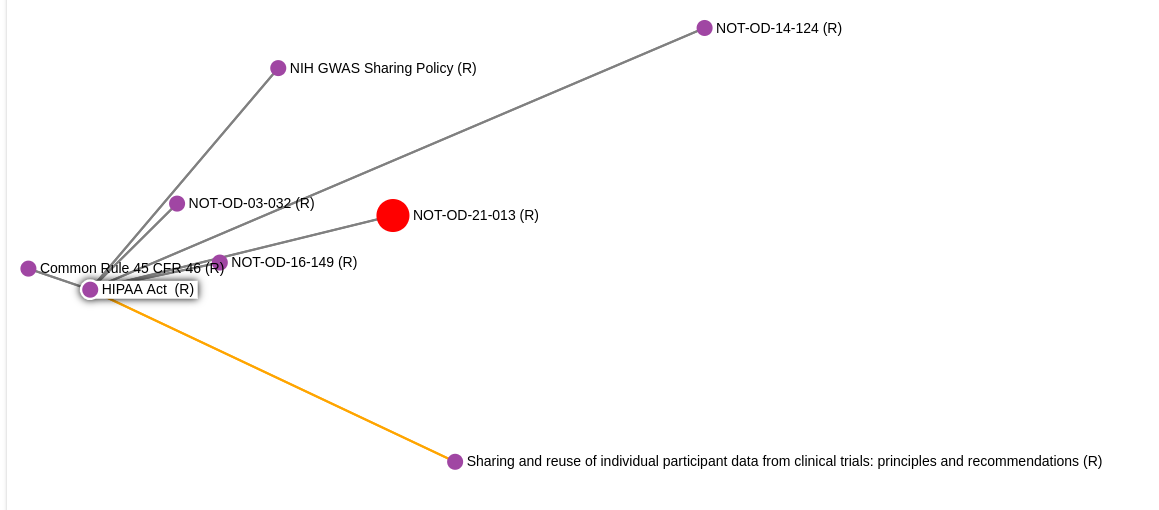
\includegraphics[width=0.9\textwidth]{FAIRSharing_NIHPol_relations.png}
    \caption{
    Grafo de uso políticas relacionadas con la política del NIH
    % \footnotemark[\ref{nih_policy_fairsharing}]
    - FAIRSharing obtenido desde \url{https://fairsharing.org/graph/4190} el 26/06/2025
    }
    \label{fairsharing_nih_policy_relations}
\end{figure}
\begin{figure}[h]
    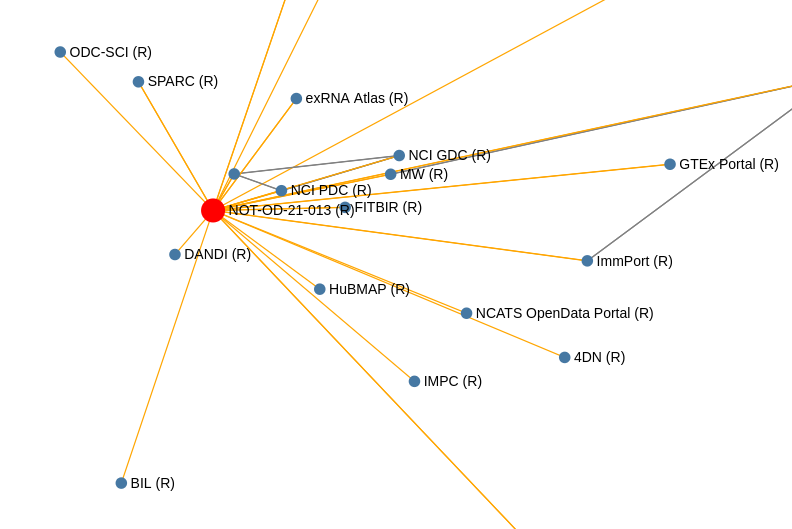
\includegraphics[width=0.9\textwidth]{FAIRSharing_NIHPol_Repos.png}
    \caption{
    Grafo de uso repositorios que utilizan la política del NIH
    % \footnotemark[\ref{nih_policy_fairsharing}]
    - FAIRSharing obtenido desde \url{https://fairsharing.org/graph/4190} el 26/06/2025
    }
    \label{fairsharing_nih_policy_repo_usages}
\end{figure}

\begin{figure}
    \centering
    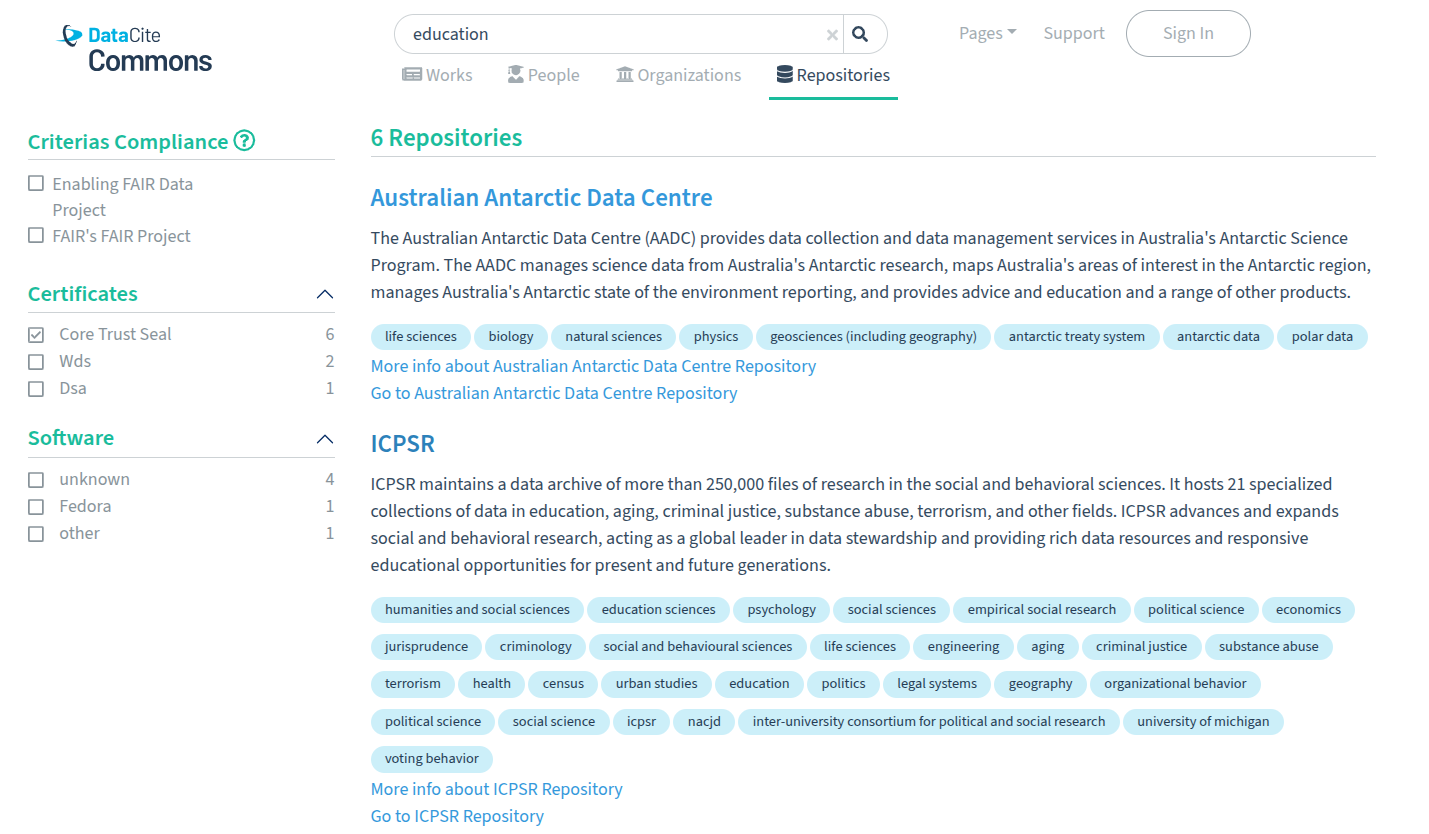
\includegraphics[width=0.5\linewidth]{datacite_commons_gral_search.png}
    \caption{Búsqueda general de repositorios de investigación en educación filtrando en base a las certificaciones disponibles 
    \footnote{\url{https://commons.datacite.org/repositories?query=education&certificate=CoreTrustSeal}}
    - Obtenido desde DataCite Commons el 26/06/2025}
    \label{fig:datacite_commons_gral_search}
\end{figure}

\begin{figure}
    \centering
    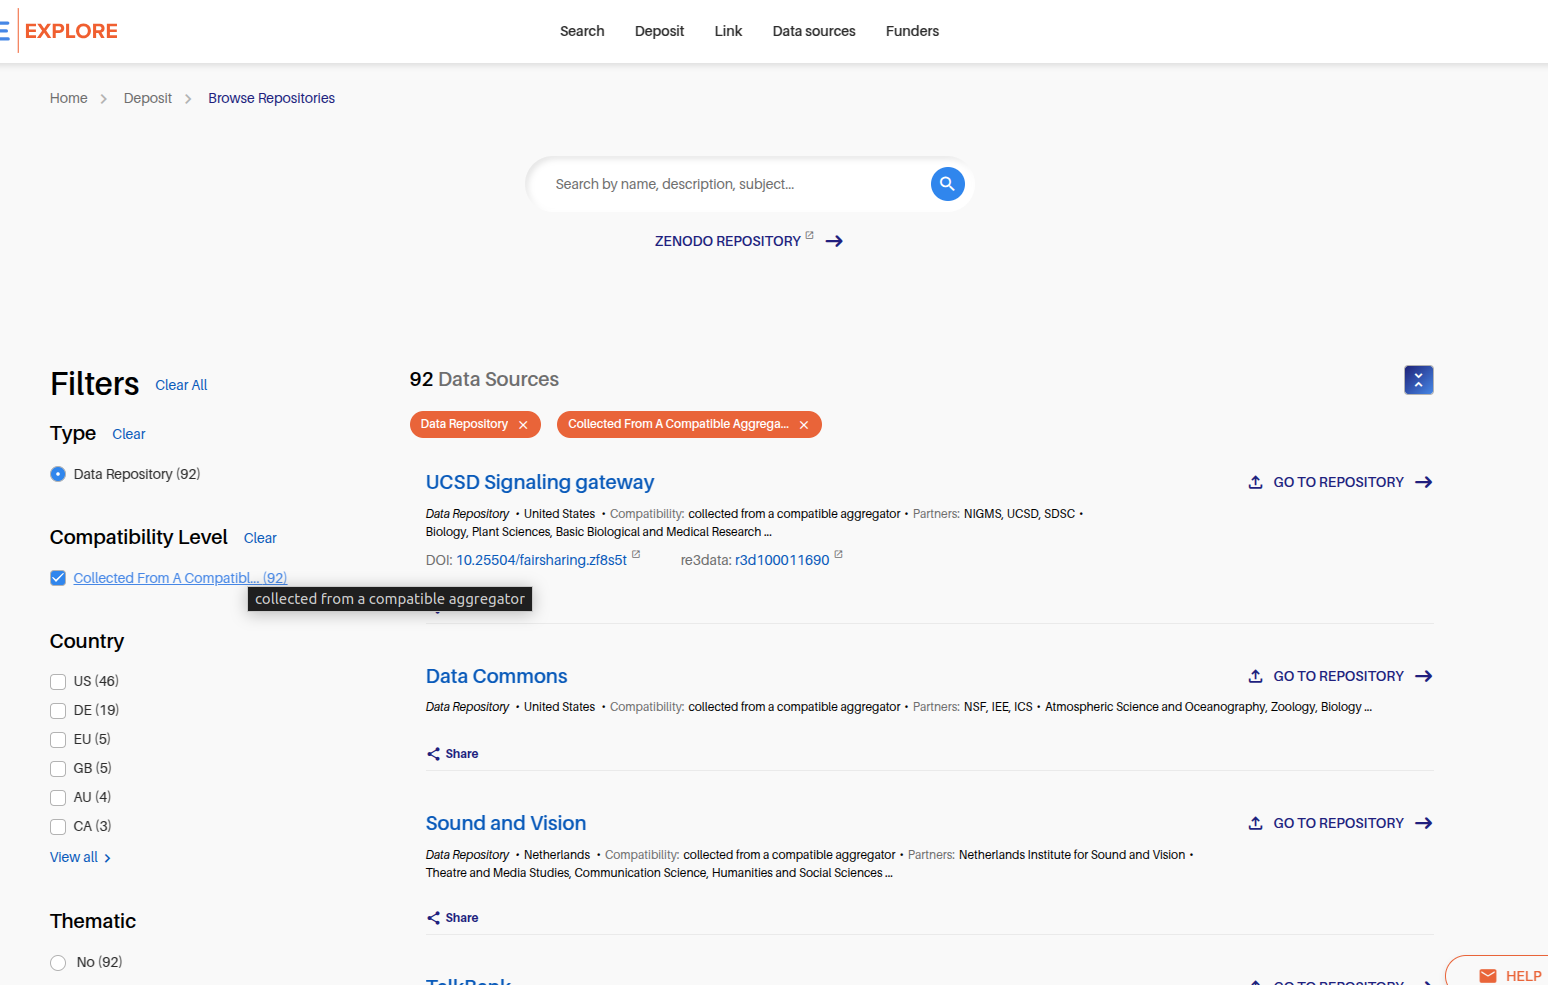
\includegraphics[width=0.5\linewidth]{openaire_gral_search.png}
    \caption{
Busqueda general de repositorios de datos de instigación certificados y con cierto nivel de compatibilidad con la EOSC.
    \footnote{\url{https://explore.openaire.eu/search/find/datasources}}
    - Obtenido desde OpenAIRE el 26/06/2025
    }
    \label{fig:openaire_gral_search}
\end{figure}

\begin{figure}
    \centering
    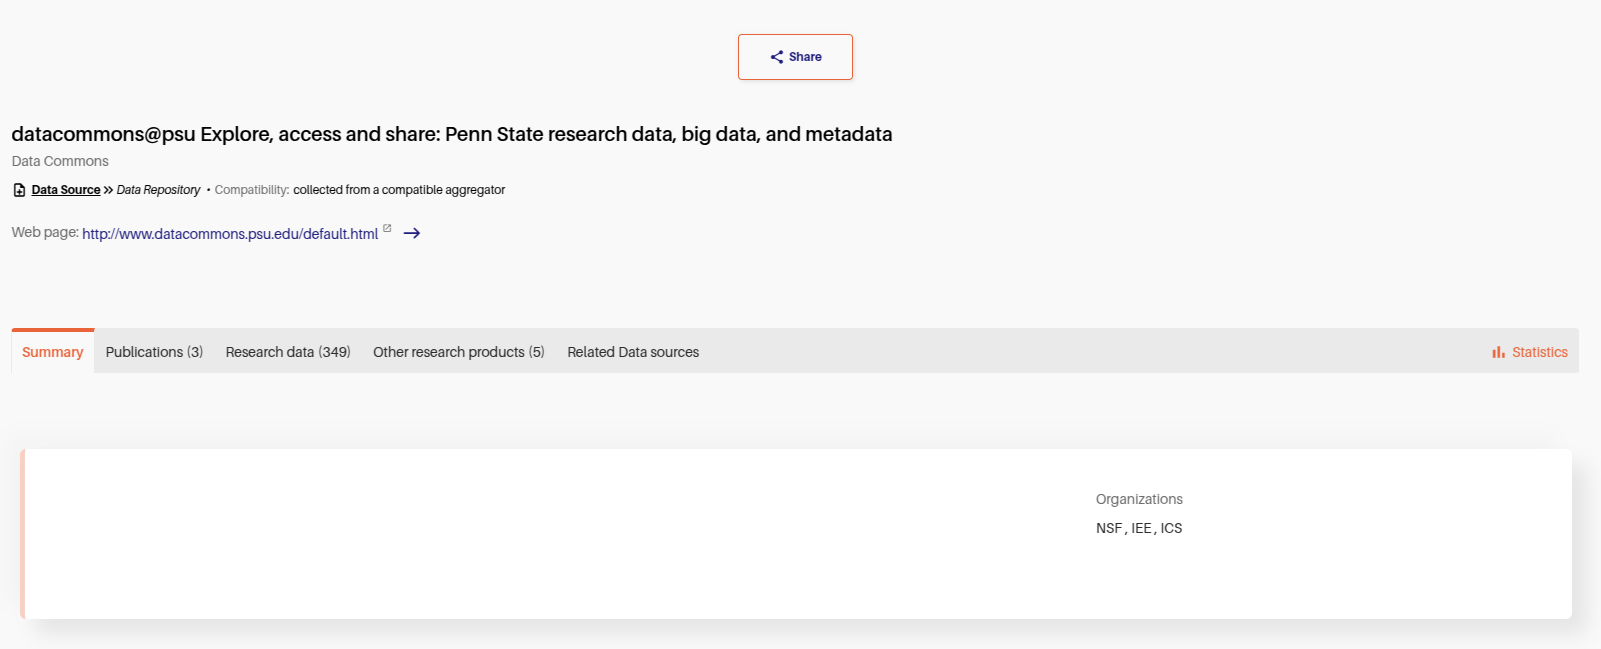
\includegraphics[width=0.5\linewidth]{repositorio_openaire.png}
    \caption{Descripción de un repositorio - OpenAIRE Explore - Obtenido el 26/02/2025}
    \label{fig:repositorio_openaire}
\end{figure}

\begin{figure}
    \centering
    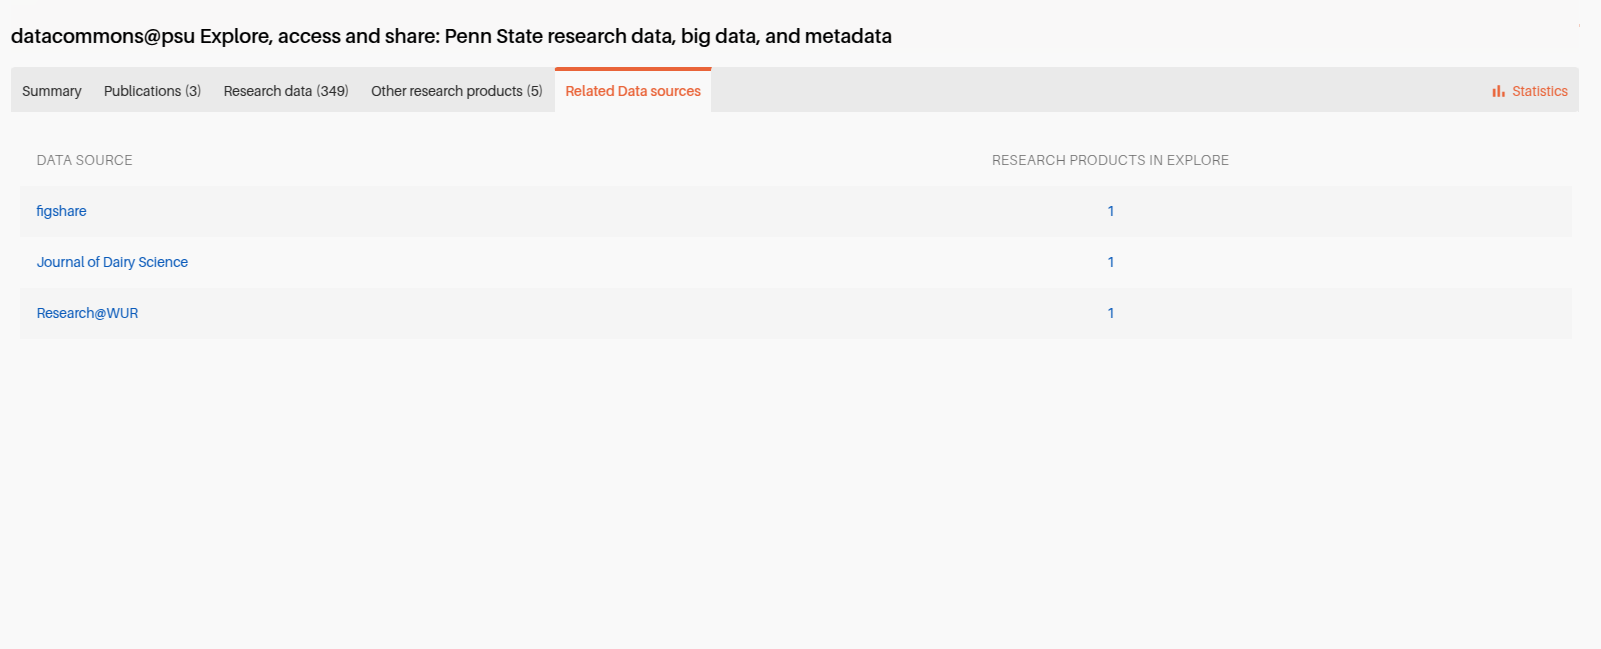
\includegraphics[width=0.5\linewidth]{openaire_recursos_relacionados_a_repositorio.png}
    \caption{Recursos y servicios relacionados al repositorio - OpenAIRE Explore - Obtenido el 26/02/2025}
    \label{fig:openaire_recursos_relacionados_a_repositorio}
\end{figure}


La presencia de certificaciones es una manera sencilla de evaluar la sostenibilidad de los repositorios u otros aspectos políticos, así como también el uso de buenas prácticas a nivel técnico. Las certificaciones son estándares de calidad que evaluan aspectos como sostenibilidad, preservación y accesibilidad de un repositorio. El otorgamiento de estos es un proceso que suele ser conducido por instituciones confiables especializadas en repositorios como CoreTrustSeal \footnote{\url{https://www.coretrustseal.org/}} \bchgon mencionar TRUST?\echgon, y garantizan en cierta medida que esos estándares fueron logrados. Los catálogos de repositorios, como FAIRSharing, ayudan a entender las implicaciones más importantes de cada tipo de certificación sin necesidad de conocer los mecanismos por los cuales se logran.\\

\begin{figure}
    \centering
    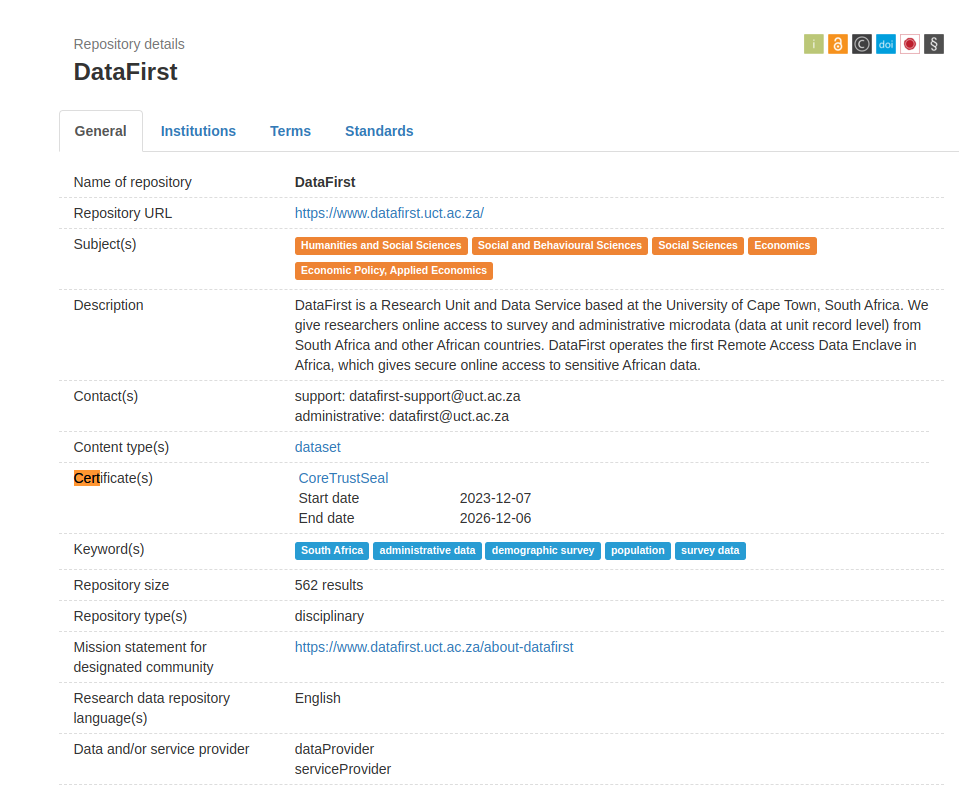
\includegraphics[width=0.5\linewidth]{re3data_certified_repo.png}
    \caption{Repositorio como es desplegado donde se muestra declaradas sus certificaciones - re3data - Obtenido el 26/02/2025}
    \label{fig:re3data_certified_repo}
\end{figure}

\begin{figure}
    \centering
    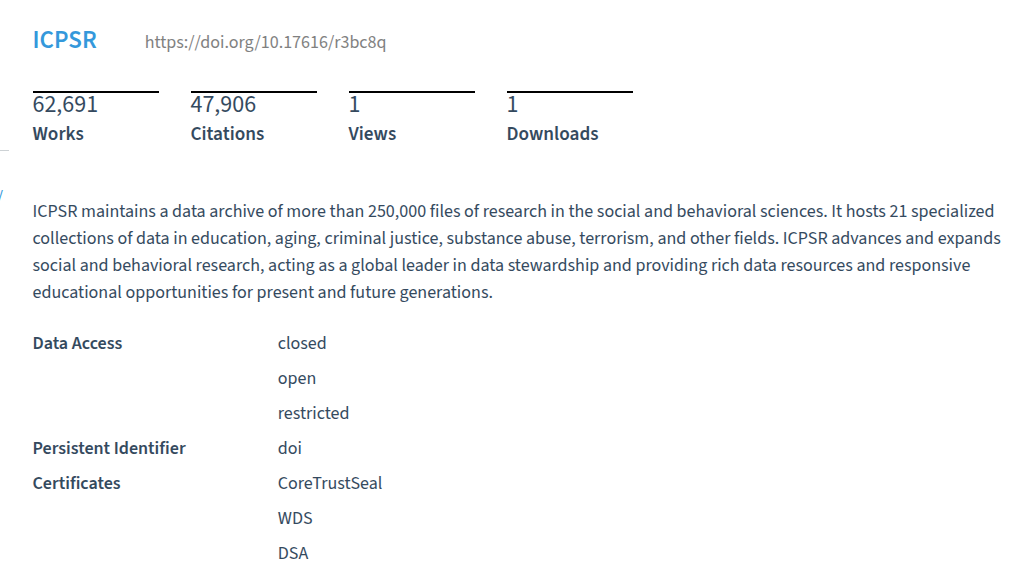
\includegraphics[width=0.5\linewidth]{datacite_certified_repo.png}
    \caption{Repositorio como es desplegado donde se muestra declaradas sus certificaciones - DataCite Commons - Obtenido el 26/02/2025}
    \label{fig:datacite_certified_repo}
\end{figure}

\begin{figure}
    \centering
    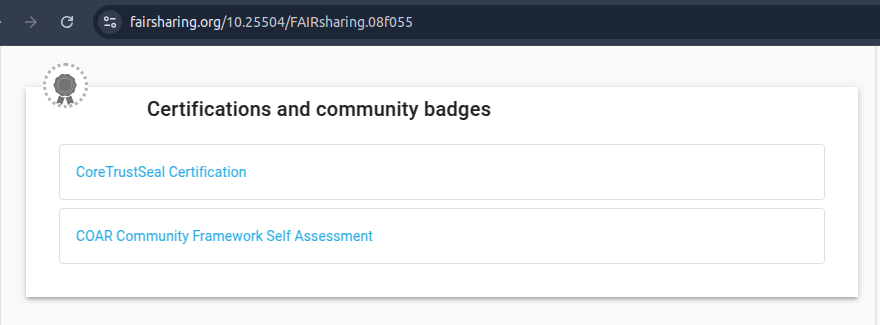
\includegraphics[width=0.5\linewidth]{fairsharing_certified_repo.png}
    \caption{Repositorio como es desplegado donde se muestra declaradas sus certificaciones - FAIRSharing - Obtenido el 26/02/2025}
    \label{fig:fairsharing_certified_repo}
\end{figure}

\begin{figure}
    \centering
    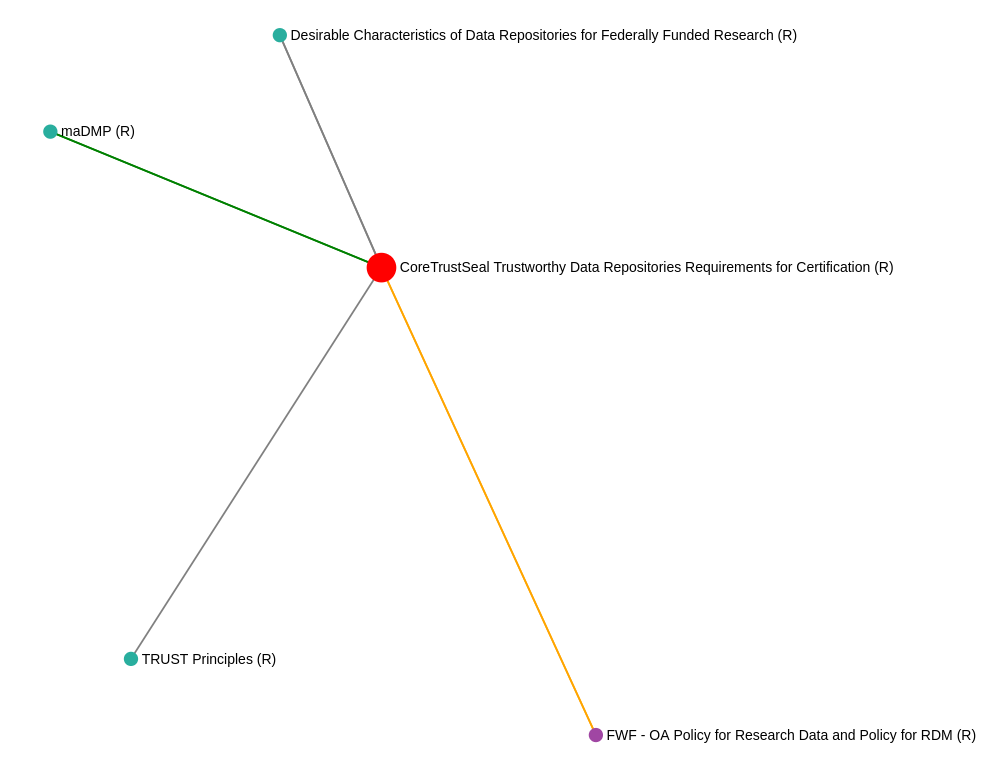
\includegraphics[width=0.5\linewidth]{certificates_relations.png}
    \caption{Representación gráfica de la certificación CoreTrusSeal y sus relaciones con otros políticas, estándares y certificaciones - FAIRSharing - Obtenido el 26/02/2025}
    \label{fig:certificates_relations}
\end{figure}

Las relaciones de los repositorios con diferentes instituciones también son desplegadas de manera oportuna y pueden servir para evaluar la sostenibilidad o las políticas asociadas. Catálogos como re3data (\ref{re3data_institutions}) o FAIRSharing (\ref{fairsharing_institutions}) proveen una visión clara de estas relaciones de manera resumida y centralizada.\\

\begin{figure}
    \centering
    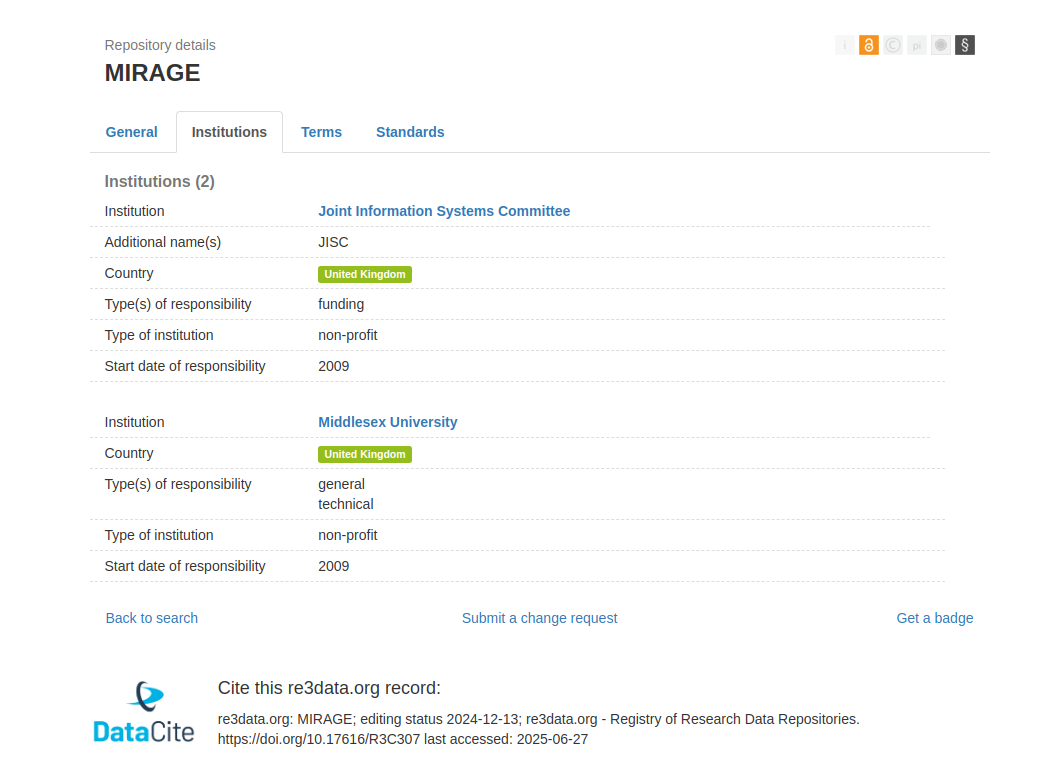
\includegraphics[width=0.5\linewidth]{re3data_institutions.png}
    \caption{instituciones relacionadas con un repositorio con sus correspondientes roles - re3data - Obtenida el 26/02/2025}
    \label{fig:re3data_institutions}
\end{figure}

\begin{figure}
    \centering
    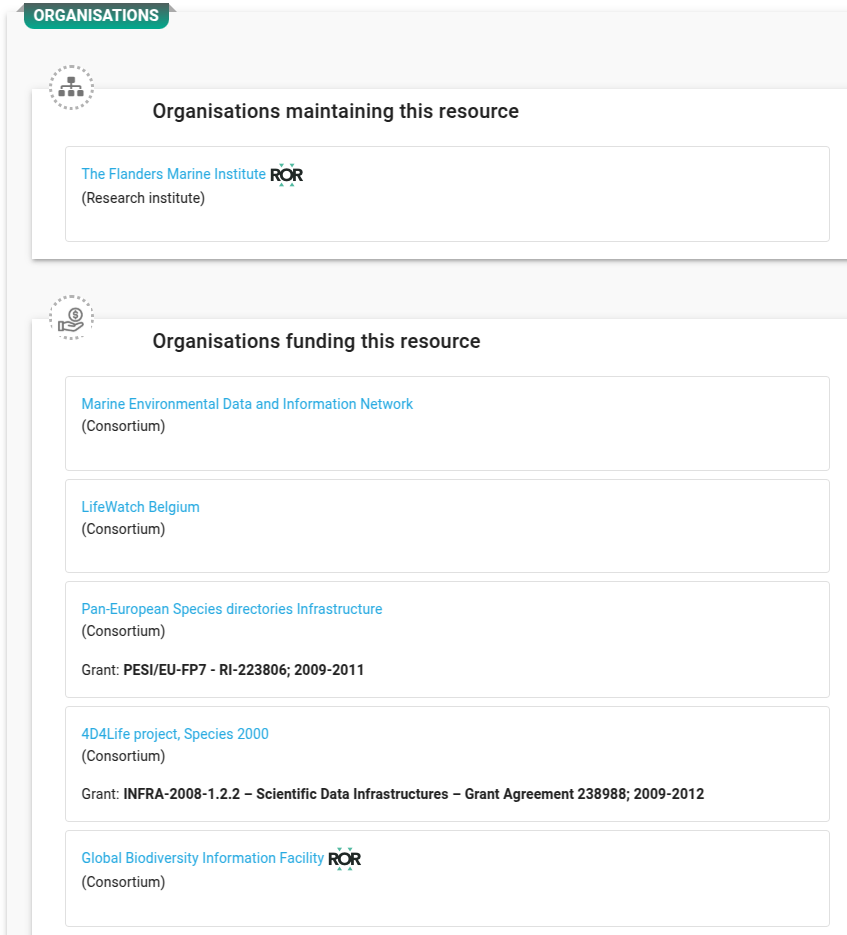
\includegraphics[width=0.5\linewidth]{fairsharing_institutions.png}
    \caption{instituciones relacionadas con un repositorio con sus correspondientes roles - FAIRSharing - Obtenida el 26/02/2025}
    \label{fig:fairsharing_institutions}
\end{figure}

Conocer el nivel de actividad que un repositorio presenta,  por ejemplo, la popularidad del repositorio en relación a ciertos tipos de contenidos, puede ayudar a ratificar que el repositorio esté funcionando correctamente. Algunos catálogos como DataCite Commons ofrecen estadísticas de uso de cada repositorio (mostrado en \ref{fig:datacite_commons_histograma}), como un modo de evaluar rápidamente la vigencia del mismo o el uso que su comunidad está haciendo de él.\\

\begin{figure}
    \centering
    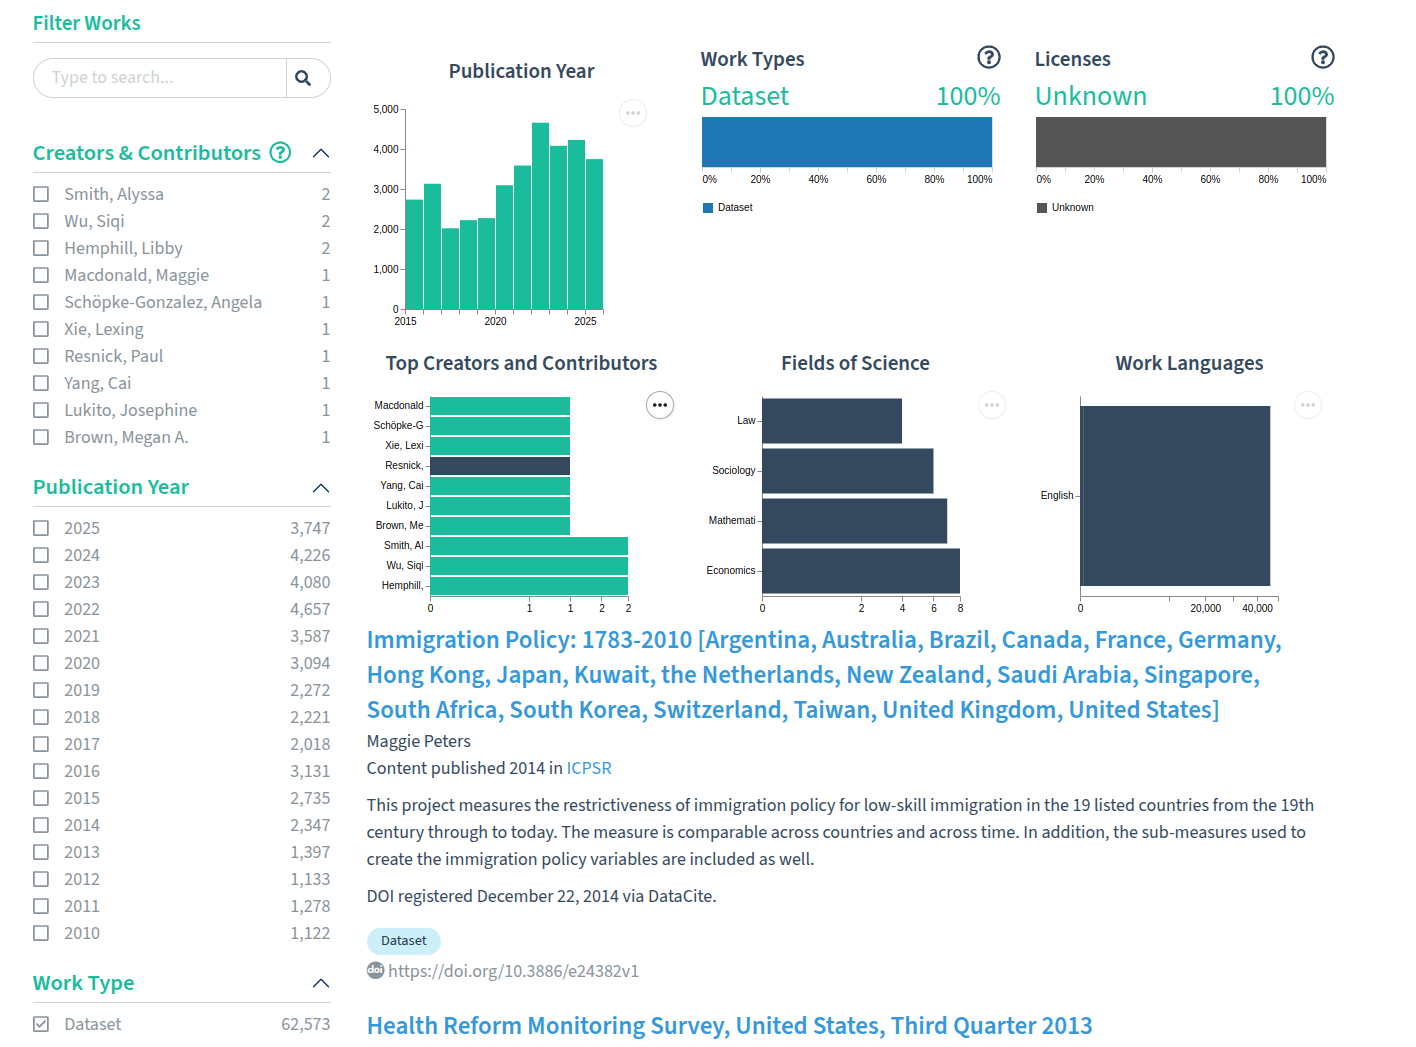
\includegraphics[width=0.5\linewidth]{datacite_commons_histograma.png}
    \caption{Histograma de contenidos del ICPSR 
    \footnote{\url{https://commons.datacite.org/repositories/gesis.icpsr?resource-type=dataset}}
    - Obtenido desde DataCite Commons el 26/06/2025}
    \label{fig:datacite_commons_histograma}
\end{figure}

Conocer la capacidad del repositorio para proveer o integrarse con ciertos servicios especializados en el área de investigación, así como las condiciones bajo las cuales los provee (precio del servicio o el nivel de disponibilidad del servicio), puede resultar decisivo para los investigadores.  
Para enumerar algunos de estos servicios y funcionalidades se pueden mencionar la capacidad de realizar o recibir revisiones formales, la posibilidad de establecer períodos de embargo, asistencia técnica especializada o la disponibilidad de servicios de curaduría disciplinar.\\
En particular, para el caso de repositorios de datos de investigación cualitativos, la presencia o integración de servicios como anonimización, o mecanismos de control de acceso resulta valiosa para los investigadores del área de ciencias sociales. 
Catálogos como OpenAIRE ofrecen información sobre la integración de los diferentes repositorios con el ecosistema de servicios de la EOSC (Amnesia\footnote{\url{https://www.openaire.eu/amnesia-guide}}, OpenAIRE AAI \footnote{\url{https://catalogue.openaire.eu/service/openaire.aai/overview}}, Argos \footnote{\url{https://catalogue.openaire.eu/service/openaire.argos/overview}}, Zenodo \footnote{\url{https://zenodo.org/}}), mediante el uso de su platafoma de \textit{linking}\footnote{\url{https://www.openaire.eu/linking}}.\\
\bchregi Tenes algun ejemplo de como lo muestra? se puede hacer una captura de pantalla y insertarlo aqui como una figura.
\echregi \\
\bchgon
Bien, te entendí
\echgon

\bchgon
TENGO que poner algo sobre la capacidad de los repositorios para menejar información contextual.
\echgon

La falta de repositorios disciplinares o comunitarios no evidencia la falta de una comunidad activa, sin embargo, es importante convenir estándares locales, que, fuera del escenario ideal, facilitan la convergencia paulatina a un estándar común, para eso es imperativo que las prácticas de gestión de datos estén más extendidas como elemento transversal en las diferentes comunidades científicas. Construír y compartir estas decisiones
\bchregi que decisiones? \echregi
\bchgon convenciones a las que puede llegar una comunidad. vamos a usar tal software en común, tales reglas y guías para nombrar las datos, etc. ¿Quizás la palabra acuerdos o convenciones es más adecuada? \echgon
mediante vocabularios controlados, taxonomías u otros objetos semánticos es una práctica más frecuente en varias disciplinas que aumenta las posibilidades de reutilización de los datos generados.\\

%\echgon

\section{Discusion}
\bchedel A continuación, se presenta un análisis de la adecuación de la información provista por los catálogos, para la evaluación de la calidad de los repositorios por parte de los investigadores. Este análisis se basa en los atributos de calidad identificados a partir de la revisión bibliográfica y consulta a experto.    \echedel \\
%%%%%%%%%%%%%%%%%%%%%%%%%%%%%%%%%%%%%%%%%%%%%%  
\bchregi  Presentar como hallazgos que engloban los problemas encontrados respecto a su correspondencia con lo que ofrecen los repositorios.) \\

La revisión bibliográfica permitió identificar varios factores que influyen en la elección de repositorios por parte de los investigadores. Entre ellos, se destacan:

\begin{itemize}
    \item \textbf{Reputación del repositorio}: Los investigadores tienden a preferir repositorios con buena reputación y reconocimiento dentro de su comunidad científica. ESTO PORQUE MAPEA CON LA NECESIDAD DE RECONOCIMIENTO.
    \item \textbf{Facilidad de uso}: La interfaz del repositorio debe ser intuitiva y fácil de navegar, tanto para depositar como para acceder a los datos. ESTO PORQUE MAPEA CON LA NECESIDAD DE MENOS ESFUERZO \bchedel usabilidad? \echedel.
    \item \textbf{Disponibilidad de metadatos}: La existencia de metadatos completos y bien estructurados es crucial para facilitar la búsqueda y el descubrimiento de los datos.ESTO PORQUE MAPEA CON LA NECESIDAD DE CONTEXTUALIZAR LOS DATOS.
    \item \textbf{Cumplimiento de los principios FAIR}: Los repositorios que cumplen con los principios FAIR (Encontrables, Accesibles, Interoperables, Reutilizables) son altamente valorados, ya que garantizan la accesibilidad y la reutilización de los datos.
    \item \textbf{Servicios de preservación a largo plazo}: Los investigadores buscan repositorios que aseguren la preservación de sus datos a lo largo del tiempo, garantizando su disponibilidad futura. \bchedel esto seria sostenibilidad o sostenibilidad? \echedel
    \item \textbf{Apoyo técnico}: Un buen soporte técnico, que incluya documentación clara y asistencia personalizada, es fundamental para facilitar el uso del repositorio.ESTO PORQUE MAPEA CON LA NECESIDAD DE MENOS ESFUERZO.
\end{itemize}

%%%%%%%%%%%%%%%%%%%%%%%%%%%%%%%%%%%%%%%%%%%%%%%%%%%%%%%%%%%%%%%%%

\bchedel
para mi aca no queda bien que estos atributos de calidad que estan a continuacion se superpongan con los anteriores, porque para encabezar la lista anterior se dijo "La revisión bibliográfica permitió identificar varios factores que influyen en la elección de repositorios por parte de los investigadores...", entonces creo que habría que sintetizar los factores que se identificaron\\
\echedel
\bchgon
Edel, ¿cual es la diferencia entre los factores y los atributos de calidad?
\echgon \bchedel Creo que estamos hablando de lo mismo, pero me parece que màs bien son atributos de calidad, porque factores me parece muy genèrico  \echedel

\begin{itemize}
    \item \textbf{Fiabilidad}: El repositorio debe cumplir con estándares y principios establecidos, como los principios FAIR, y contar con una estructura de gobierno clara y políticas transparentes.
    \item \textbf{Cumplimiento de los principios FAIR}: El repositorio debe proporcionar metadatos claros y admitir la interoperabilidad entre diferentes formatos de datos.
    \item \textbf{Reputación y reconocimiento}: El repositorio debe gozar de buena reputación dentro de la comunidad científica y contar con el respaldo de organizaciones profesionales o instituciones académicas.
    \item \textbf{Infraestructura técnica}: El repositorio debe contar con una infraestructura sólida en términos de capacidad de almacenamiento, seguridad de los datos y protocolos de respaldo.
    \item \textbf{Documentación y soporte al usuario}: El repositorio debe proporcionar documentación completa y un buen soporte técnico para facilitar su uso.
    \item \textbf{Sostenibilidad}: El repositorio debe contar con un modelo de financiación a largo plazo y un plan para garantizar su funcionamiento continuo y contempla planes de continuidad para evitar perdida de información.
\end{itemize}
\echregi

\section{Conclusiones y Trabajos futuros}

Este trabajo se desarrolló en el contexto de la investigación educativa y la publicación de datos de investigación asociados a esta área. Se reconoce que la investigación educativa comparte varias características con la investigación en general en lo que respecta a la gestión de datos, pero también presenta desafíos específicos relacionados con la heterogeneidad de los datos y las restricciones éticas y legales.\\

El análisis realizado subraya la importancia de abordar las necesidades de los investigadores en relación con los repositorios de datos. Se identificó que la interoperabilidad, el apoyo institucional y la asistencia técnica son aspectos cruciales para la comunidad investigadora. Además, se constató un desconocimiento generalizado sobre las opciones disponibles de repositorios de datos, a pesar de que los investigadores reconocen la importancia de las prácticas de publicación de datos.\\

Es importante destacar la apertura de los investigadores hacia la publicación de datos y su reconocimiento de los beneficios que esto conlleva tanto para quienes publican como para quienes acceden a los datos. Sin embargo, las herramientas tecnológicas actuales no parecen ofrecer una solución integral que cubra todas las necesidades de los investigadores educativos en materia de publicación de datos.\\

A pesar de esta limitación, el estudio permitió realizar una evaluación comparativa de los catálogos de repositorios de datos de investigación. En este sentido, \textbf{FAIRSharing} se destaca como la herramienta que ofrece los mejores niveles de curaduría y calidad de datos. También se resalta su modelo de sostenibilidad y la transparencia de sus criterios y procesos. \textbf{FAIRSharing} proporciona una visión orgánica del proceso de publicación y de la infraestructura de investigación abierta. Debido a que la base de datos de \textbf{FAIRSharing} carece de algunos registros, se recomienda realizar una consulta paralela en \textbf{Repository Finder}.\\

En cuanto a la evolución de las tecnologías para la catalogación de repositorios, \textbf{re3data}, si bien sigue cumpliendo un rol fundamental como fuente primaria de información, ha sido superado por herramientas que ofrecen una mejor usabilidad e interoperabilidad.\\

En conclusión, este estudio proporciona información valiosa para los investigadores educativos que buscan publicar sus datos de investigación. Al destacar los factores clave que influyen en la elección de repositorios y al evaluar las características de los catálogos de repositorios disponibles, se busca facilitar la toma de decisiones informadas y promover una mayor adopción de prácticas de datos abiertos en el campo de la investigación educativa.\\

\bchgon
- Sobre la utilidad de los catálogos de repositorios.\\
  - Hay aún mucho que mejorar en cuánto a la capacidad de los repositorios para informar sobre sus características.
  - La idea de repositorio como objeto definido, así como el proceso de publicación tiene actualmente ha sido moldeado desde una perspectiva mucho más centrada en la gestión de los datos que en las visión de utilidad de los investigadores. Aún existe una gran brecha entre estas dos visiones.
  - Nombrar a los PGD como una herramienta que recoge en un documento las visiones de ambos actores

- La necesidad de apoyo institucional debería ser uno de los outputs\\

- No hay actualmente maneras sencillas de visualizar la interconexión entre repositorios y comunidades que permita la difusión de los datos a un público particular\\

- Los investigadores difícilmente puedan evaluar nociones de calidad tan complejas como la sostenibilidad de un repositorio, que depende de factores técnicos y políticos difíciles de resumir o de estimar a largo plazo. Para esto, es necesario dar voz a las recomendaciones y advertencias de expertos de manera imparcial. Las certificaciones cumplen un papel fundamental, pero la infraestructura que las sustenta aún puede mejorar para ser más transparente.\\

- Como concuerdan varios autores en https://meetingorganizer.copernicus.org/EGU24/EGU24-20387.html, es necesario mejorar la capacidad de descubrimiento de los repositorios y servicios disponibles en la infraestructura de investigación.

- Para la sección de mejoras a futuro se puede citar a https://zenodo.org/records/10847707 donde se propone la potenciar e interconectar los recursos dados por los catálogos mediante la web semantica. O en FAIR 2.0 según https://scispace.com/papers/fair-2-0-extending-the-fair-guiding-principles-to-address-2sa0tfp53f \\
\echgon

\bibliographystyle{apalike}
\bibliography{sample}

\end{document}
